\documentclass[aps,prb,
%,twocolumn
,floatfix,footinbib,longbibliography,
preprint
]{revtex4-1}
%\documentclass[aps,preprint,floatfix,footinbib,longbibliography]{revtex4-1}
\usepackage{epsfig}
\usepackage{graphicx}% Include figure files
\usepackage{dcolumn}% Align table columns on decimal point
\usepackage{bm}% bold math
\usepackage{mathrsfs}
\usepackage{amsmath}
\usepackage{bbold}
\usepackage{color}
\usepackage{epstopdf}
\usepackage{subfigure} 
%\usepackage[backend=bibtex,sorting=none,style=trad-abbrv,citestyle=numeric]{biblatex}

%\usepackage[sorting=none]{biblatex}
%\usepackage{hyperref}
%\usepackage[titletoc]{appendix}
% avoids incorrect hyphenation, added Nov/08 by SSR
\hyphenation{ALPGEN}
\hyphenation{EVTGEN}
\hyphenation{PYTHIA}

\usepackage[colorlinks=true,pdfborder=001,linkcolor=blue,anchorcolor=blue,citecolor=blue,urlcolor=blue]{hyperref}

\newcommand{\revision}[1]{{\color{blue}{#1}}}



\begin{document}

%\preprint{APS/123-QED}

%\title{Electron-hole pair excitation and energy transport in hybrid electron-boson junctions}
%\title{Electron-hole pair excitation and unified description of hybrid energy transport in electron-boson nano-junctions}

%\title{Charge transfer electron-hole pair excitation and energy transport in hybrid electron-boson nano-junctions}

\title{Nonequilibrium reservoir engineering of a biased coherent conductor for hybrid energy transport in nanojunctions}

% \title{Hybrid electron-boson system as a electron-hole pair exciton reservoir}

\author{Bing-Zhong Hu}
%\author{Tao Wang}
\author{Lei-Lei Nian}
\email{llnian@hust.edu.cn}
\author{Jing-Tao L\"{u}}
\email{jtlu@hust.edu.cn}
\affiliation{School of Physics and Wuhan National High Magnetic Field Center, Huazhong University of Science and Technology, Wuhan 430074, P. R. China}


\date{23 March, 2019}% It is always \today, today,%but any date may be explicitly specified
\begin{abstract}
%We propose a Landauer-B\"uttiker formula to describe  energy transport between weakly coupled hybrid electron-boson nano-junctions. The electron bath is described by effective bosonic baths with possibly nonzero chemical potential.  Our theory gives a unified account of current-induced heating/cooling, electroluminescence and thermoelectric transport in nano-junctions. Our results extend the Landauer formalism to hybrid electron-boson systems and shed light on the nature of energy transfer between electron and boson systems.

%We show that a current-carrying coherent electron conductor can be treated as effective bosonic energy reservoir involving different types of electron-hole pair excitation. Hybrid energy transport between nonequilibrium electrons and bosons can be described by a Landauer-B\"uttiker formula. This allows for intuitive and unified account of a variety of heat transport problems in hybrid electron-boson systems, including non-reciprocal heat transport between electrons and bosons, thermoelectric current from a cold-spot and radiative cooling. 
We show that a current-carrying coherent electron conductor can be treated as effective bosonic energy reservoir involving different types of electron-hole pair excitation. For weak electron-boson coupling, hybrid energy transport between nonequilibrium electrons and bosons can be described by a Landauer-like formula. This allows for unified account of a variety of heat transport problems in hybrid electron-boson systems. As applications, we study the non-reciprocal heat transport between electrons and bosons, thermoelectric current from a cold-spot and electronic cooling of the bosons.
Our unified framework provides an intuitive way of understanding hybrid energy transport between electrons and bosons. It opens the way of nonequilibrium reservoir engineering for efficient energy control between different quasi-particles in the nanoscale.


%Our results extend the Landauer formalism to hybrid electron-boson systems and shed light on the nature of energy transfer between electron and boson systems.

%Our theory paves the way of designing hybrid quantum devices for efficient energy control in the nanoscale.
%\begin{description}
%\item[PACS numbers]
%73.63.Kv, 73.23.-b, 71.38.-k, 72.25.-b
%\end{description}
\end{abstract}


\maketitle
%\tableofcontents

%\section{Introduction-1}
%Chemical potential is a key concept in thermodynamics and statistical mechanics. As the conjugated variable to the particle number, chemical potential difference drives particle transport or chemical reactions.

\section{Introduction}
%\emph {Introduction.--} 
%20200223--------------------------------------
%Understanding nonequilibrium energy transport in the nanoscale is of crucial importance both for the fundamental development of quantum thermodynamics and for the practical application of nanoscale thermal, thermoelectric and optoelectronic devices. Energy carriers following different statistics, including electrons\cite{imry1999conductance}, photons\cite{ojanen2008mesoscopic,biehs2010mesoscopic,zhang2018energy,benabdallah2014near}, phonons\cite{rego1998quantized,mingo2005carbon,yamamoto2006nonequilibrium,wang2006nonequilibrium,wang2007nonequilibrium,wang2008quantum,ruokola2009thermal,li2012colloquium,taylor2015quantum,wang2016landauer} and magnons\cite{wang2004spin}, have been used for the control of nanoscale energy transport. Theoretical approaches developed for each quasi-particle can be readily applied in these studies.
%20200223--------------------------------------

Understanding nonequilibrium energy transport in the nanoscale is of crucial importance both for the fundamental development of quantum thermodynamics and for the practical application of nanoscale thermal, thermoelectric and optoelectronic devices. For phase coherent transport, the celebrated Landauer-B\"uttiker formalism has been successfully applied to study quasi-particle energy transport following different statistics, including electrons\cite{imry1999conductance}, photons\cite{ojanen2008mesoscopic,biehs2010mesoscopic,zhang2018energy,benabdallah2014near}, phonons\cite{rego1998quantized,mingo2005carbon,yamamoto2006nonequilibrium,wang2006nonequilibrium,wang2007nonequilibrium,wang2008quantum,ruokola2009thermal,li2012colloquium,taylor2015quantum,wang2016landauer} and magnons\cite{wang2004spin}.
%The energy current between two baths ($i=1,2$) can be written as the following general form
%\begin{equation}
%J_{}=\int_{0}^{+\infty}\frac{d\omega}{2\pi}\hbar\omega T(\omega)[n_{}(\omega,\mu_{1},T_{1})-n_{}(\omega,\mu_{2},T_{2})].
%\label{eq:lb}
%\end{equation}
Wherein, the baths connecting to the system are assumed to be in thermal equilibrium with given temperature and/or chemical potential, where the quasi-particle distribution function  is determined by its statistics, i.e., the Fermi-Dirac distribution for fermions, and the Bose-Einstein distribution for bosons. A difference in the distribution drives an energy current flow between the two thermal baths. 

%This driving force for energy transport could be a chemical potential or temperature bias for fermions. However, for bosons we have $\mu=0$ in thermal equilibrium, following the textbook argument that bosons without number conservation have zero chemical potential. Thus, for bosonic energy transport the only driving force is temperature.


%Here, the transmission coefficient $T(\omega)$ describes the transmission probability of particle with energy $\hbar\omega$. The distribution function $n(\omega,\mu,T)$ is determined by the particle statistics. It is the Fermi-Dirac distribution for fermions. Either a chemical potential or a temperature bias can drive an energy current flow. Thus, thermoelectric transport can also be studied using this equation. For bosons, $n$ is the Bose-Einstein distribution. Equation~\ref{eq:lb} has been used to study temperature-driven bosonic energy transport carried by phonons, photons and other quasi-particles. Here, we have $\mu=0$, following the textbook argument that bosons without number conservation have zero chemical potential. Thus, for bosonic energy transport the only driving force is temperature.

However, the same approach is difficult to describe energy transport between quasi-particles following different statistics, which is ubiquitous in thermoelectric and optoelectronic processes of nano-junctions. Examples of such processes include electroluminescence\cite{kuhnke2017atomic,galeprin2017photonics,schneider2010optical,schneider2012light}, Joule heating\cite{huang2007local,ioffe2008detection,lu_current-induced_2015,hartle2011resonant,hartle2011vibrational,hartle2018cooling}, current-induced\cite{galperin2009cooling,simine2012vibrational,lykkebo2016single,hartle2011resonant} or radiative cooling\cite{zhu2019near}. Another difficulty arising in these processes is that the quasi-particles may be in nonequilibrium state due to driving from external bias.

In this work, we show that these processes can be conveniently analyzed by `bosonizing' a voltage-biased coherent electron conductor into bosonic reservoir with non-zero chemical potential. In the limit of weak electron-boson coupling, we obtain a Landauer formula to describe energy transport between electrons and bosons. This is possible since energy transport between electrons and bosons is always accompanied by the generation or annhilation of different kinds of electron-hole pairs (EHPs)\cite{headgordon_molecular_1995,dou2018perspective}. We thus generalizes the Landauer formalism to hybrid energy transport between possibly nonequilibrium baths, and provides a unified framework to understand energy transport in different thermal, thermoelectric and optoelectronic processes.  

%However, the generation and annihilation of bosons may be accompanied by transitions between different states of particles with non-zero chemical potentials. This is certainly the case for electrically driven processes. In such situations, it is known that the chemical potential of bosons does not have to be zero. In this work, we show that, energy transport between steady-state nonequilibrium electrons and bosons can be well described by a Landauer-B\"uttiker formula between bosonic baths with different chemical potentials. The key observation is that, the electronic system can be treated as bosonic electron-hole-pair bath with a non-zero chemical potential. This general formula can give a unified account of different physical processes involving energy transfer between fermionic and bosonic systems, including current-induced heating/cooling, electrically-driven light emission and thermoelectric transport in nano-scale junctions.







%\begin{align}
%n_{\alpha}(\omega,\nu_{\alpha},T_{\alpha})=\frac{1}{e^{\beta_\alpha(\hbar\omega-\mu_{\alpha})}-1}
%\end{align}
% is the Bose-Einstein
%distribution function in bath $\alpha (=1, 2)$ with the inverse temperature $\beta_\alpha=(k_BT_{\alpha})^{-1}$, $k_B$ being the Boltzmann constant. We have included the chemical potential $\mu_{\alpha}$, which is normally set to zero for phonon or photon transport.

\section{Theory}
\subsection{System setup}
%\subsection{Model}
%\emph{Model.--} 
We consider a model system schematically shown in Fig.~\ref{fig:ehp} (a). The \emph{system} composed of an independent set of bosonic degrees of freedom (DOF) taken as a set of harmonic oscillators. It couples to two kinds of baths. One is an equilibrium boson bath (ph-bath), modeled by an infinite number of harmonic oscillators (bosonic modes). The other is an electron bath (e-bath), which itself includes a central part ($C$) and two electrodes ($L$ and $R$).  The e-bath may be driven into a nonequilibrium steady state by a voltage bias applied between the two electrodes. Without loss of generality, we assume that the system couples only to the central region of the e-bath. Energy transport between the two baths takes place through their simultaneous coupling to the system. 
%We limit ourselves to non-interacting electrons and weak electron-boson interaction such that a lowest order expansion is valid\cite{paulsson05modeling}. Extension to interacting electrons is possible\cite{dou_born-oppenheimer_2017}. 
The electrons couple to the `displacement' of the system harmonic oscillators
\begin{equation}
H_{es} = \sum_{i,j,k} M^{k}_{ij}c^\dagger_i c_j u_k.
\label{eq:eboson}
\end{equation}
Here, $M^k_{ij}$ describes the coupling of the system mode $k$ to the electronic transition between states $i$ and $j$, and $u_k$ is the `displacement' operator of the system mode $k$. For phonons, it is the displacement, while for photons it is the vector potential. The system-ph-bath coupling is linear between harmonic oscillators and can be treated exactly.

%The above model is quite general. 

%To be more specific, we consider a molecular conductor as an example. of the e-bath. The system is then made of harmonic vibrations of the molecule. The electrode phonons can serve as the ph-bath. Thus, the model introduced here can be used to study energy transport in molecular conductors\cite{lu2007coupled,lu2011laserlike,lu2016electron}.

%Applications of this model include current-induced heating or electroluminescence. The bosonic system represents molecular vibrations and cavity photon modes, respectively. 


\subsection{Electron-hole pair excitation}
%\emph{ Electron-hole pair excitation.--}
Our key observation is that the energy transport between the system and the e-bath can be modeled by different kinds of reactions between EHPs in the e-bath and the bosonic modes in the system. The creation and annihilation of the bosonic mode is always accompanied by the recombination and creation of EHPs. These processes can be expressed in the form of reactions
\begin{align}
e_\alpha + h_\beta \rightleftharpoons b_n,
\label{eq:reaction}
\end{align}
where $e_\alpha$, $h_\beta$ and $b_n$ represent electron in electrode $\alpha$, hole in electrode $\beta$ and bosonic mode $b_n$ in the system. Equivalently, we can write 
\begin{align}
e_\alpha \rightleftharpoons e_\beta + b_n,
\label{eq:reaction2}
\end{align}
representing inelastic electronic transition from electrode $\alpha$ to $\beta$, accompanied by emission of bosonic mode $n$ (forward process). The backward direction corresponds to absorption process.


There are four types of EHPs which we label by the spatial location of the electron ($\alpha$) and hole  ($\beta$) states. They are schematically shown in Fig.~\ref{fig:ehp} (c) and (d) for recombination and creation processes, respectively. They are denoted by EHP-$i$ ($i=1,2,3,4$) and are further divided into two groups. The intra-electrode type includes $1/LL$ and $2/RR$, and inter-electrode type includes $3/RL$, $4/LR$.  Additional to energy transfer between e-bath and system, the generation and recombination of inter-electrode EHPs also involves charge transport across the system. We take the energy of mode  and the EHPs to be positive. 


A generalized detailed balance relation applies to each of reactions
\begin{align}
\frac{\tau _{\alpha\rightharpoonup\beta}}{\tau_{\alpha\leftharpoondown\beta}} = {\rm exp}\left[-\beta_B(\hbar\Omega-\mu_{\alpha\beta})\right].
\label{eq:db}
\end{align}
Here, $\tau_{\alpha\rightharpoonup\beta}$ and $\tau_{\alpha\leftharpoondown\beta}$ are the reaction rates for the forward (boson emission) and backward (boson absorption) processes in Eq.~(\ref{eq:reaction}), respectively. They are obtained from the Fermi golden rule
\begin{align}
\tau_{\alpha\rightharpoonup\beta} &= \frac{2\pi}{\hbar}\sum_{i\in\alpha,f\in\beta}|M^m_{ij}|^2  \delta(\varepsilon_i-\varepsilon_f-\hbar\Omega)  \nonumber\\
&\times n_F(\varepsilon_i-\mu_\alpha)(1-n_F(\varepsilon_f-\mu_\beta)).
\end{align}
Here, $n_{F/B}(\varepsilon,T) = \left[{\rm exp}\left(\beta_B \varepsilon\right)\pm 1\right]^{-1}$ is the Fermi-Dirac/Bose-Einstein distribution, with $\beta_B=(k_BT)^{-1}$,  $\mu_{\alpha\beta}=\mu_\alpha-\mu_\beta$, and $M^m_{ij}=\langle \psi_{i}(\varepsilon_i)|M^{}|\psi_{f}(\varepsilon_f)\rangle$ is the transition matrix element from initial state $i$ in electrode $\alpha$ to final state $f$ in electrode $\beta$. The reverse rate $\tau_{\alpha\leftharpoondown\beta}$ can be written similarly.
Thus, when reaching equilibrium with the EHP bath $\alpha\beta$, the bosonic mode follows a Bose-Einstein distribution at temperature $T_e$ and chemical potential $\mu_{\alpha\beta}$. For intra-electrode processes, $\mu_{\alpha\beta}=0$, we have the normal detailed balance relation, while for inter-electrode processes $\mu_{\alpha\beta}$ is determined by the applied voltage bias. Thus, the bosonic mode may acquire a non-zero chemical potential in nonequilibrium. This is consistent with the equilibrium condition for reaction \ref{eq:reaction}.


%Non-zero chemical potential of the EHPs indicates that energy and heat are not equivalent anymore for the inter-electrode EHPs. Taking the process 4 in Fig.~\ref{fig:ehp}(c) as an example, energy conservation requires $\varepsilon_\alpha = \varepsilon_\beta +\hbar\omega_n$. Due to the finite chemical potential, the heat flowing with the boson is $Q=\hbar\omega_n-\mu_{LR}$.  Similarly, the heat flowing with bosons emitted by process 3 is $Q=\hbar\omega_n-\mu_{RL}$. For $T_e=T_{ph}$ and $\mu_{LR}>0$, we arrive at a seemingly surprising result: the total energy $\hbar\omega_n$ emitted in process 4, normally termed Joule heat, actually include some chemical work. Even more counter-intuitively, when $\mu_{LR}>\hbar\omega_n$, $Q$ becomes negative, meaning that the emitted boson carries negative entropy, which is a resource for work extraction.

\begin{figure}
	%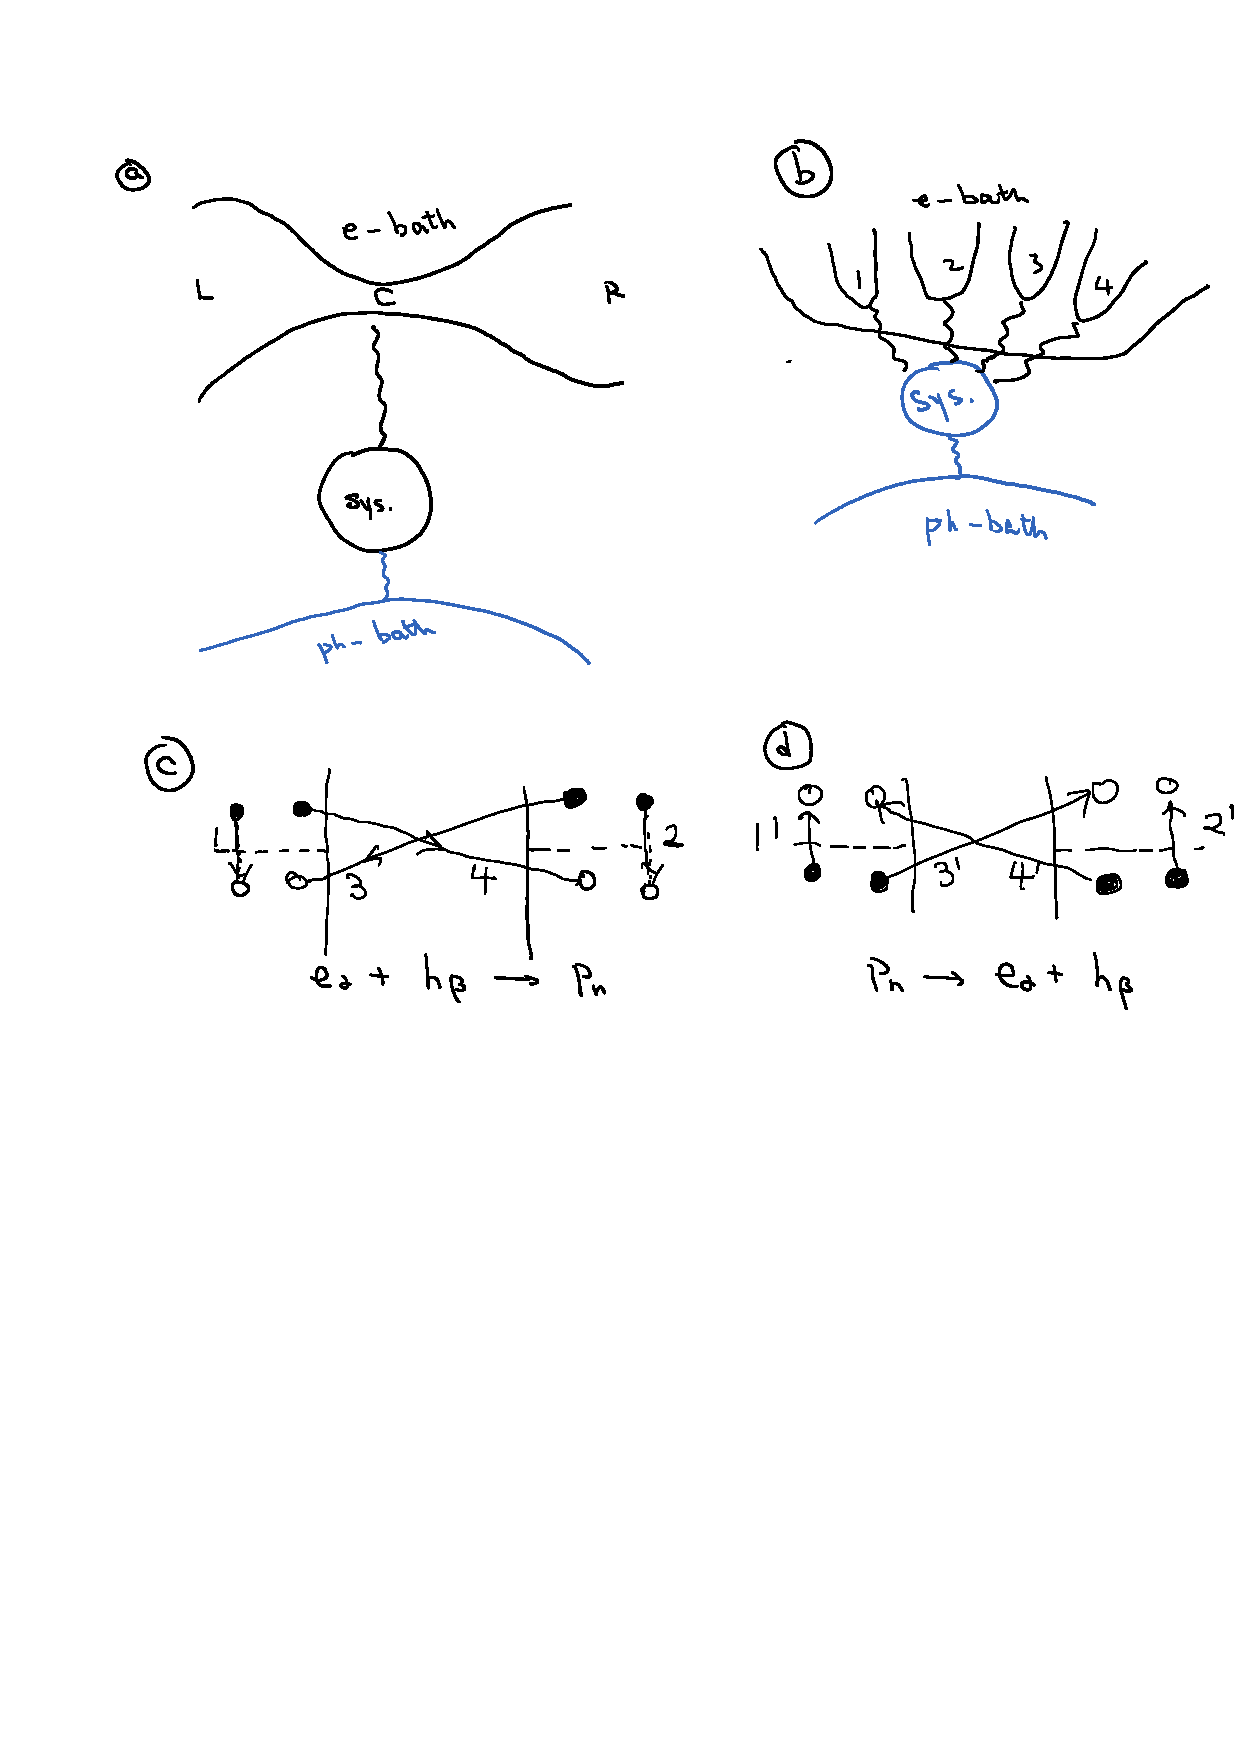
\includegraphics[scale=0.45,angle=0]{schematics-v3.pdf}		
	\centering
	\subfigure[]{
	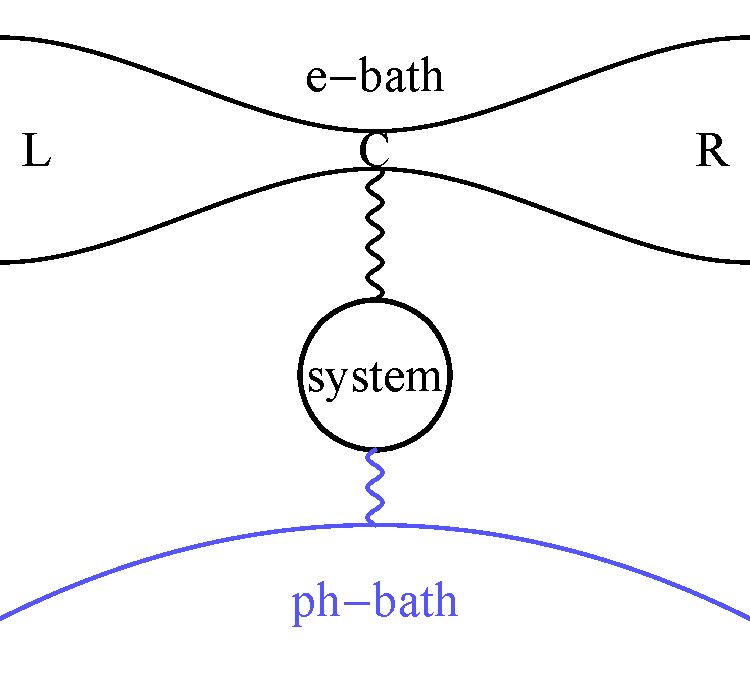
\includegraphics[width=0.2\textwidth,angle=0]{figures/fig_1a.pdf}
	%\caption{fig1}
	}
	\quad
	\subfigure[]{
	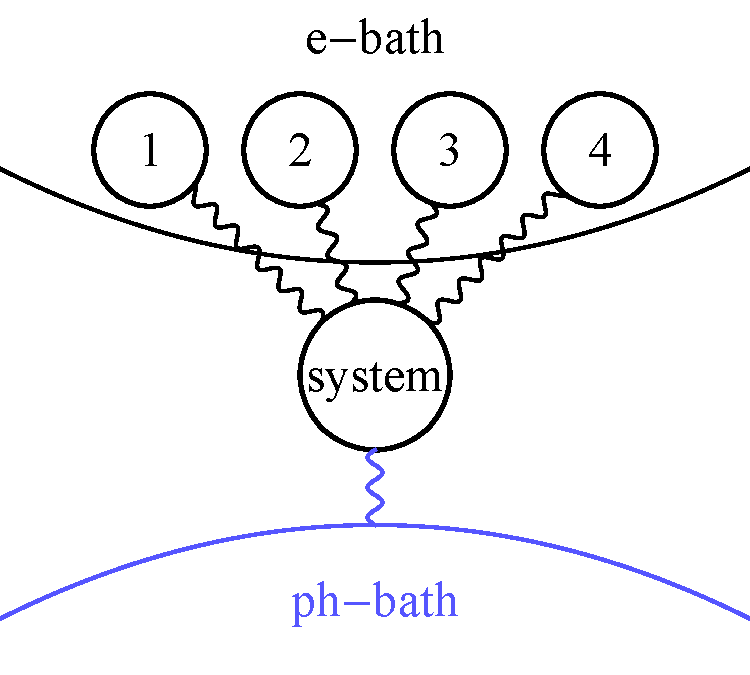
\includegraphics[width=0.2\textwidth,angle=0]{figures/fig_1b.pdf}
	}
	\quad
	\subfigure[]{
	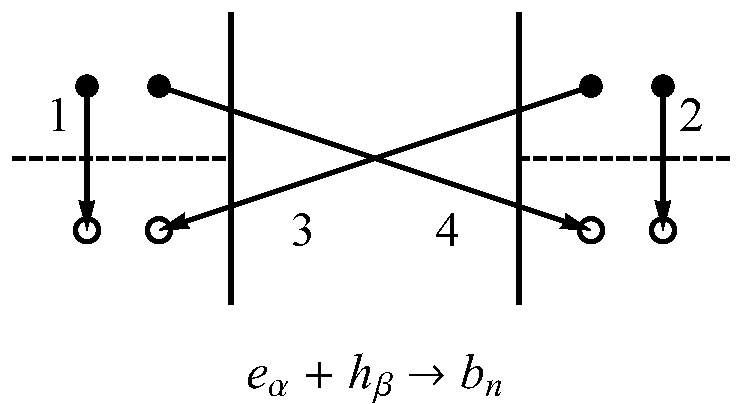
\includegraphics[width=0.2\textwidth,angle=0]{figures-0317/fig_1c.pdf}
	}
	\quad
	\subfigure[]{
	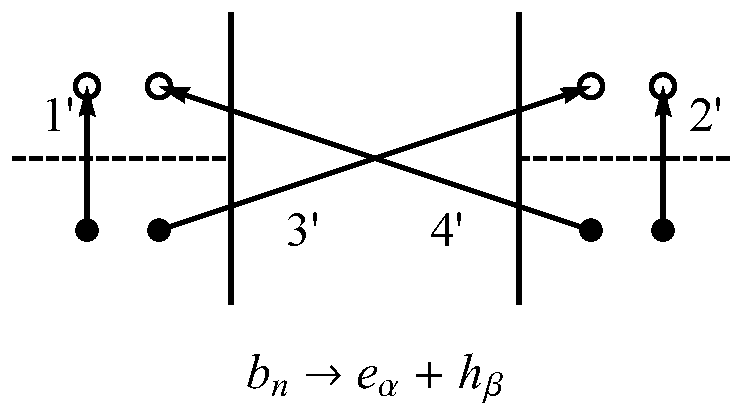
\includegraphics[width=0.2\textwidth,angle=0]{figures-0317/fig_1d.pdf}
	}
	\caption{(a) Schematics of the model we consider. The system consists a set of independent bosonic modes. It couples to an electron bath (e-bath), which is modeled as a conductor including a left (L) and a right (R) electrode, with temperature $T_e$ and chemical potential $\mu_L$ and $\mu_R$, respectively. The system further couples to an external thermal bath (ph-bath) at temperature $T_{ph}$. (b) The electron bath can be treated as four different kinds of electron-hole pair (EHP) baths (1-4), shown in (c). (c-d) Four kinds of EHP recombination (c) and excitation (d) processes. The EHPs are classified according to the spatial location of the electron ($e_\alpha$) and the hole ($h_\beta$).}
	\label{fig:ehp}
\end{figure}




%\emph{Power spectrum and energy transport.--} 
The key quantity to describe the EHP baths is the coupling-weighted power spectrum. It can be written as
\begin{align}
\tilde{\Pi}_{mn}^{\alpha\beta}(\omega) &= \left[n_B(\hbar\omega-\mu_{\alpha\beta},T_e)+\frac{1}{2}\right]\Lambda_{mn}^{\alpha\beta}(\omega).
\label{eq:ppehp}
\end{align}
We have introduced the coupling-weighted EHP density of states (DOS)\cite{lu_current-induced_2012,lu2016electron}
\begin{align}
\Lambda_{mn}^{\alpha\beta}(\omega) &= -\sum_{i\in\alpha,f\in\beta}M^{m}_{fi}M^n_{if}  \delta(\varepsilon_i-\varepsilon_f-\hbar\omega)\nonumber\\
&\times (n_F(\varepsilon_\alpha-\mu_\alpha,T_\alpha)-n_F(\varepsilon_\beta-\mu_\beta,T_\beta))\nonumber\\
&=-\int \frac{d\varepsilon}{2\pi} {\rm tr}[M^m A_\alpha(\varepsilon) M^n A_\beta(\varepsilon-\hbar\omega)] \nonumber\\
&\times (n_F(\varepsilon-\mu_\alpha,T_\alpha)-n_F(\varepsilon-\hbar\omega-\mu_\beta,T_\beta)),
\label{eq:gamma}
\end{align}
which also characterizes the system dissipation due to coupling to the e-bath\cite{lu_current-induced_2012}. Here, $A_\alpha$ is electrode spectrum functional.
Equation~(\ref{eq:ppehp}) follows a form of the fluctuation-dissipation relation for an equilibrium ph-bath, albeit with a possibly non-zero chemical potential  $\mu_{\alpha\beta}$. The intra-electrode EHPs (i=1,2) are always in equilibrium with $\mu_{\alpha\alpha}=0$ and temperature $T_e$. But the two inter-electrode EHPs (i=3, 4) have opposite chemical potential $\mu_{RL}=-\mu_{LR}$. They are non-zero when there is a voltage bias applied.  To this end, we have shown that the nonequilibrium e-bath can be divided into four EHP baths with different chemical potentials.
This effective model is shown in Fig.~\ref{fig:ehp} (b).

%\emph{Detailed balance and effective temperature.--}
%We now proceed to show that, a slightly modified detailed balance relation applies to each of the EHP baths. 
%To simplify the analysis, we consider one bosonic mode with angular frequency $\Omega$. A simple rate equation for the mode population $N$ can be established by considering the forward and backward reaction processes
%\begin{align}
%\dot{N} = B (N+1) - A N,
%\end{align}
%where $B$ and $A$ are the reaction rates for the emission and absorption of bosonic quanta, respectively. They can be calculated by summing over the individual rates $B=\sum_{\alpha\beta}B_{\alpha\beta}$, $A=\sum_{\alpha\beta}A_{\alpha\beta}$.
%, with
%\begin{align}
%B_{\alpha\beta} &= \frac{2\pi}{\hbar}\sum_{i_\alpha,f_\beta}|\langle \psi_{i}(\varepsilon_i)|M^{m}|\psi_{f}(\varepsilon_f)\rangle|^2 \\
%&\times %n_F(\varepsilon_i)(1-n_F(\varepsilon_f))\delta(\varepsilon_i-\varepsilon_f-\hbar\Omega),
%\end{align}
%and $A_{\alpha\beta}$ is obtained by the replacement $\hbar\Omega \to -\hbar\Omega$. As a result, the ratio $A/B$ follows
%The reaction rates of each EHP bath follows a generalized detailed balance relation
%\begin{align}
%\frac{A_{\alpha\beta}}{B_{\alpha\beta}} = {\rm exp}(\beta_B(\hbar\Omega-\mu_{\alpha\beta})).
%\end{align}
%with a possibly nonzero chemical potential $\mu_{\alpha\beta}=\mu_\alpha-\mu_\beta$, as required by the equilibrium condition for reaction \ref{eq:reaction}.

%This means each type of the reaction drives the mode into a Bose-Einstein with a chemical potential $\mu_{\alpha\beta}$. This coincides with the chemical potential of the corresponding EHPs, as required by the equilibrium condition of \ref{eq:reaction}:
%\begin{align}
%\mu_\alpha-\mu_\beta = \mu_p.
%\end{align}
%Here, we have used the fact that chemical potential of holes is the opposite to that of electrons.

%The bosonic mode reaches steady state when $\dot{N}=0$, with
%\begin{align}
%N = \frac{1}{A/B-1}.
%\end{align}
%In equilibrium ($\mu_\alpha=\mu_\beta$), we have $A/B={\rm exp}(\beta_B\hbar\Omega)$. When there is voltage bias applied, the final distribution can not be written as a simple form. Normally, an effective temperature is defined by assuming $N$ follows the Bose-Einstein distribution with zero chemical potential
%\begin{align}
%k_BT_{eff} = \frac{\hbar\Omega}{{\rm ln}(1+N^{-1})}.
%\end{align}
%According to previous discussion, we can equivalently defined an effective chemical potential by assuming $N$ follows the Bose-Einstein distribution at $T_e$ 
%\begin{align}
%\mu_{eff} = \hbar\Omega - k_BT{\rm ln}(1+N^{-1}).
%\end{align}
%These two effective parameters are related through
%\begin{align}
%T_{eff} = \frac{T_e}{1-\mu_{eff}/(\hbar\Omega)}.
%\label{eq:tmu}
%\end{align}
%Several comments are noteworthy at this point. Firstly, in the presence of voltage bias, if the reverse of process 4 is normally enhanced more than process 3, we have a positive $\mu_{eff}$ and consequently $T_{eff}>T_e$. The result is heating of the bosonic mode. In the limiting case shown in Fig.~(\ref{fig:resonant}) (a), resonant enhancement may lead to the extreme case of $\mu_{eff}=\hbar\Omega$, or $T_{eff}\to +\infty$. This marks the instability of the bosonic mode. This case has been analyzed in details in Ref.~\onlinecite{lu2011laserlike}. This instability means that the harmonic approximation is not applicable any more\cite{nitzan2018kinetic}. In the other limiting case (Fig.~\ref{fig:resonant}(b)), process 3 is resonantly enhanced, resulting in $\mu_{eff}>0$ or $T_{eff}<T_{e}$. In this regime, the voltage bias is used to cool the bosonic mode below $T_e$.

\subsection{Steady state mode population}
The reaction~\ref{eq:reaction} suggests that, when reaching steady state, the bosonic mode inherits the chemical potential of the EHPs. Thus, the bosonic mode may acquire a non-zero chemical potential. This is best illustrated by performing a mode population analysis. 

To simplify the analysis, we consider one bosonic mode with angular frequency $\Omega$. A simple master equation for the mode population $N$ can be established by considering the forward and backward reaction processes
\begin{align}
	\dot{N} = \sum_{\alpha\beta}\left[\tau_{\alpha\rightharpoonup\beta} (N+1) - \tau_{\alpha\leftharpoondown\beta} N\right].
\end{align}
%According to Eq.~(\ref{eq:db}), each type of the reaction drives the mode into a Bose-Einstein distribution with a chemical potential $\mu_{\alpha\beta}$. This coincides with the chemical potential of the corresponding EHPs, as required by the equilibrium condition of \ref{eq:reaction}:
%\begin{align}
%	\mu_\alpha-\mu_\beta = \mu_p.
%\end{align}
%Here, we have used the fact that chemical potential of holes is the opposite to that of electrons. 
The steady state population of mode is obtained by setting $\dot{N}=0$, which is written as
\begin{align}
	N = \frac{1}{\sum_{\alpha\beta}\tau_{\alpha\leftharpoondown\beta}/\sum_{\alpha\beta}\tau_{\alpha\rightharpoonup\beta}-1}.
\end{align}
In equilibrium ($\mu_L=\mu_R$), we obtain the standard Bose-Einstein distribution with temperature $T_e$ and zero chemical potential. When there is voltage bias applied ($\mu_L\neq\mu_R$), the final distribution can not be written as a simple form. Normally, an effective temperature $T_{\rm eff}$ is defined by assuming $N$ follows the Bose-Einstein distribution with zero chemical potential
\begin{align}
	k_BT_{\rm eff} = \frac{\hbar\Omega}{{\rm ln}(1+N^{-1})}.
\end{align}
According to previous discussion, we can equivalently define an effective chemical potential by assuming $N$ follows the Bose-Einstein distribution at $T_e$ 
\begin{align}
	\mu_{\rm eff} = \hbar\Omega - k_BT_e{\rm ln}(1+N^{-1}).
\end{align}
These are two equivalent equivalent ways of characterizing the nonequilibrium steady state of the vibrational mode. The two effective parameters are related via
\begin{align}
	T_{\rm eff} = \frac{T_e}{1-\mu_{\rm eff}/(\hbar\Omega)}.
	\label{eq:tmu}
\end{align}
Several comments are noteworthy at this point. Firstly, in the presence of voltage bias, if the emission process is enhanced more than the absorption process, we have a negative $\mu_{\rm eff}$ and consequently $T_{\rm eff}>T_e$. The result is heating of the bosonic mode. In the limiting case shown in Fig.~\ref{fig:resonant}(a), resonant enhancement may lead to the extreme case of $\mu_{\rm eff}=\hbar\Omega$, or $T_{\rm eff}\to +\infty$. This marks the instability of the bosonic mode. This case has been analyzed in details in Ref.~\onlinecite{lu2011laserlike}. The instability means that the perturbative analysis is not applicable any more\cite{nitzan2018kinetic}. It can be avoided by introducing additional coupling to the ph-bath. The validity of $T_{\rm eff}$ in this case will be analyzed elsewhere\cite{Wang-preprint}. In the other limiting case (Fig.~\ref{fig:resonant}(b)), the absorption process is resonantly enhanced, resulting in $\mu_{\rm eff}>0$ or $T_{\rm eff}<T_{e}$. In this regime, the voltage bias is used to cool the bosonic mode below $T_e$.

%When $eV=\hbar\Omega$, a laser-like instability occurs\cite{lu2011laserlike}. This indicates the failure of our harmonic lowest order analysis\cite{nitzan2018kinetic}.

%Efficiency of a heat engine using the bononic system as working medium
%\begin{align}
%\eta = 1-\frac{T_L}{T_H}\frac{\hbar\Omega-\mu_{eff}}{\hbar\Omega}>1-\frac{T_L}{T_H}.
%\end{align}
%It seems that the efficiency is larger than the Carnot efficiency between $T_L$ and $T_H$. The reason is that, the bosonic mode has a nonzero chemical potential, the energy input from $T_H$ includes not only heat, but also chemical energy. All the chemical energy can be converted to work.

\subsection{Energy transport}
%\emph{ Energy transport.--}
Within this effective EHP model, hybrid energy transport between  electrons and system bosons can be treated as bosonic transport.
To the lowest order approximation, we arrive at a  Landauer-like formula for the energy and particle transport from e-bath to the system as a summation of contributions from all the EHP baths
\begin{align}
J &= \sum_{\alpha,\beta}\int_0^{+\infty}\frac{d\omega}{2\pi}\hbar\omega\ {\rm Tr}[\Lambda^{\alpha\beta}(\omega)\mathcal{A}_{ph}(\omega)]\nonumber\\
&\times [n_B(\omega-\mu_{\alpha\beta},{T}_{e})-n_B(\omega,T_{ph})].
\label{eq:jjtrans}
\end{align}
%\begin{align}
%I^{ph} &= \sum_{\alpha,\beta}\int_0^{+\infty}\frac{d\omega}{2\pi}\ {\rm Tr}[\Lambda^{\alpha\beta}(\omega)\mathcal{A}_{ph}(\omega)]\nonumber\\
%&\times [n_B(\omega-\mu_{\alpha\beta},{T}_{e})-n_B(\omega,T_{ph})].
%\label{eq:iphtrans}
%\end{align}
Here, $J$ is the energy flux from e-bath to ph-bath. $T_{\rm e}$ and $T_{\rm ph}$ are the temperature of the e-bath and ph-bath, respectively. The trace Tr is over system DOF, with $\mathcal{A}_{\rm ph}$ the spectral function of the system due to coupling to the ph-bath. We can write it in terms of the non-interacting boson Green's function $D^{r/a}$ and self-energy $\Pi_{\rm ph}^{r/a}$ as $\mathcal{A}_{ph}=iD^r(\Pi_{\rm ph}^r-\Pi_{\rm ph}^a)D^a$\cite{lu2016electron}. The summation over $\alpha\beta$ includes contributions from all the four types of EHPs. Each of them contributes to one transport channel. 




%where
%\begin{align}
%\mathcal{T}^{\alpha\beta}(\omega)=
%\end{align}
%is the transmission between the EHP bath $\alpha\beta$ and the ph-bath. 

\begin{figure}[h]
	%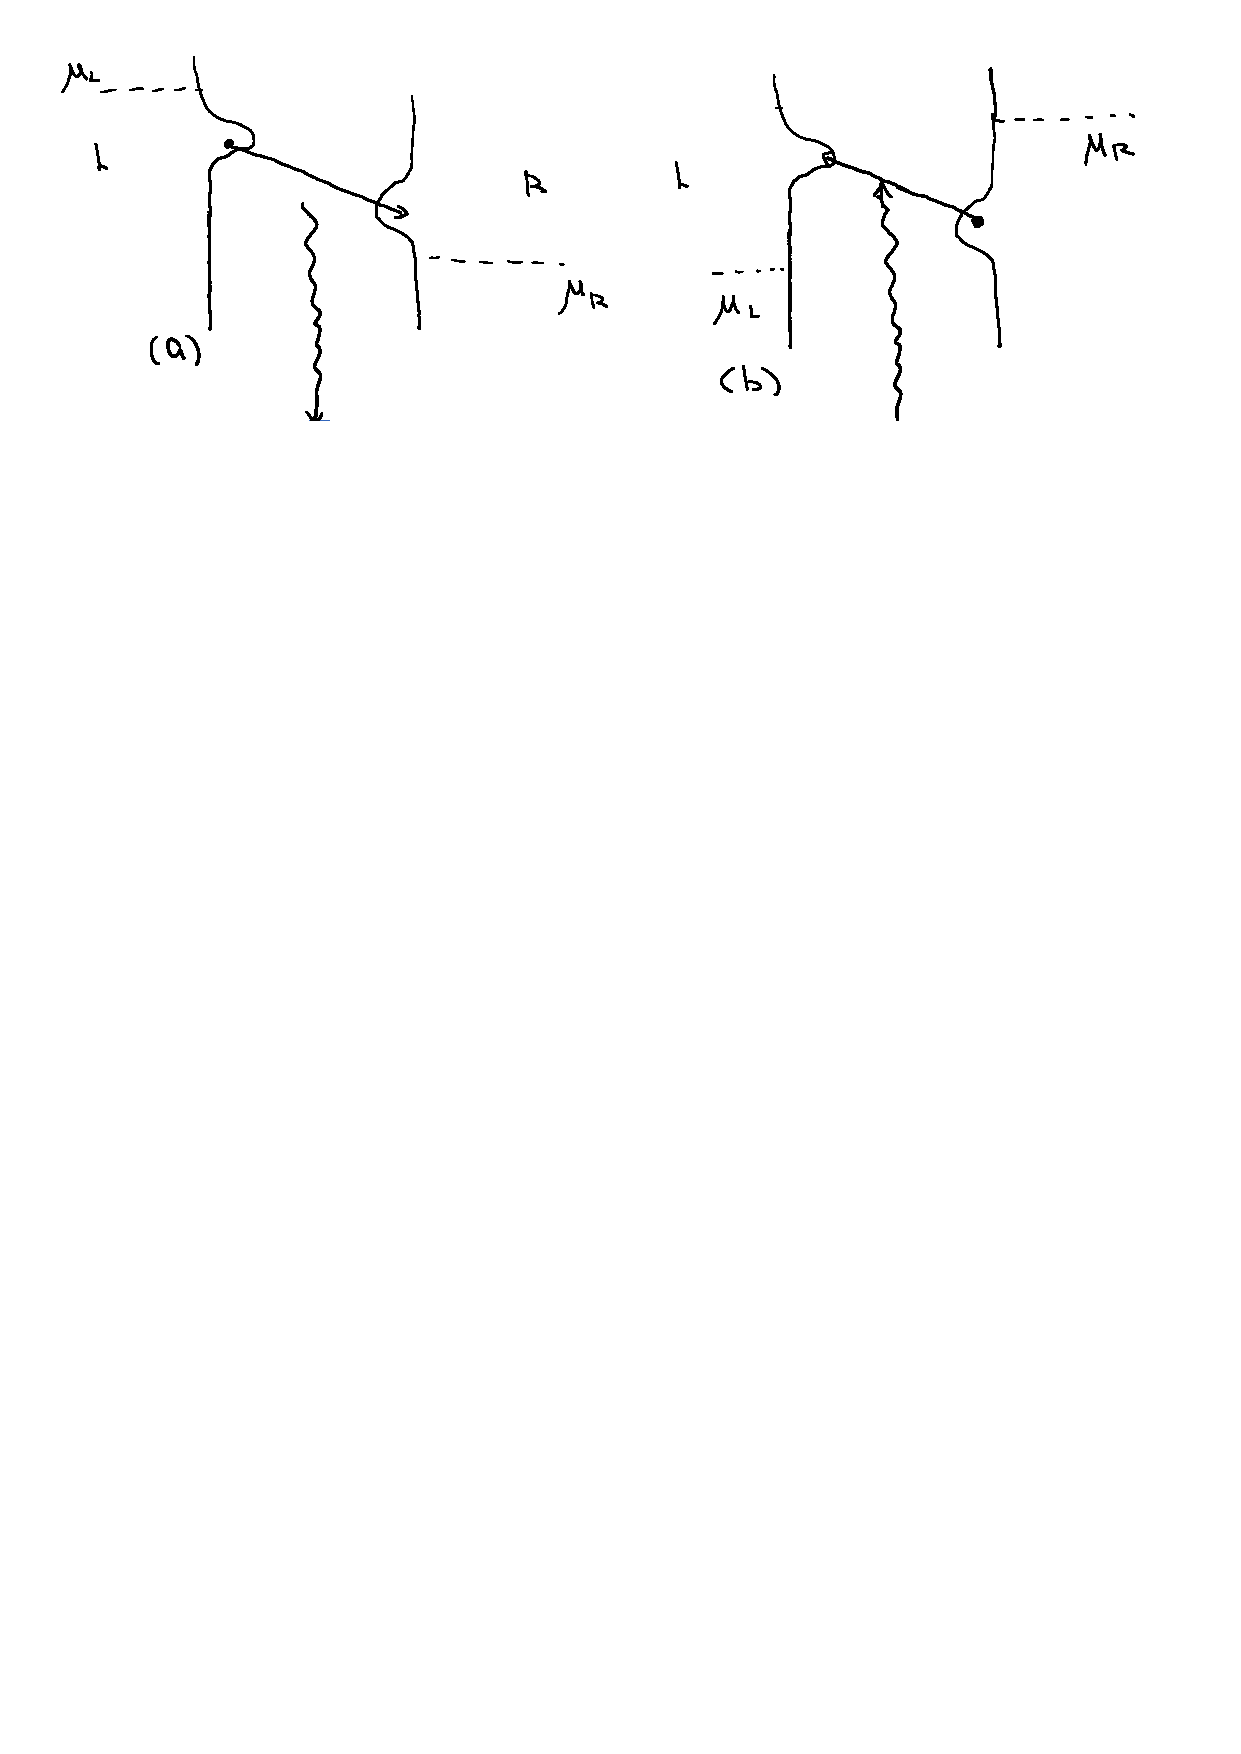
\includegraphics[scale=0.5,angle=-0]{heating-cooling-v4.pdf}
	\centering
	\subfigure[]{
		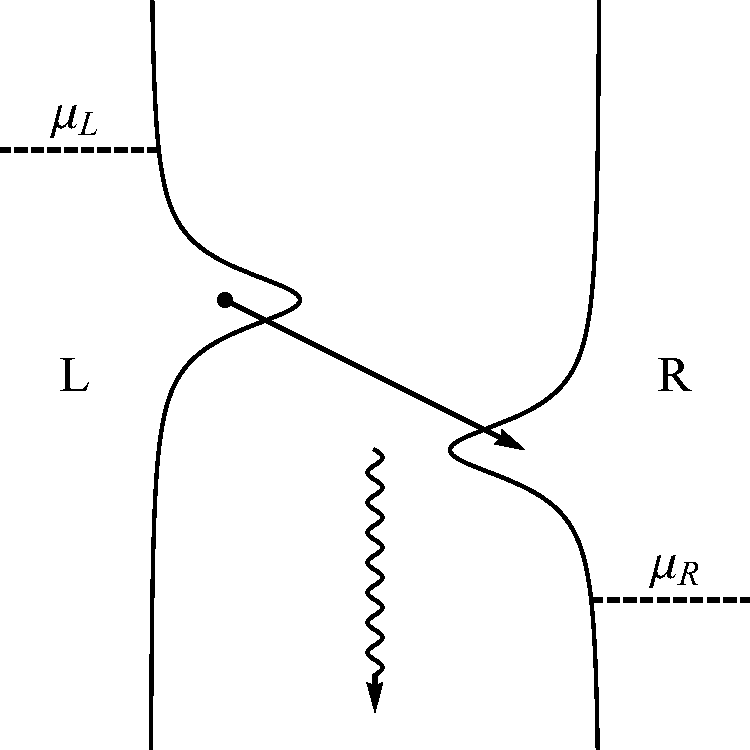
\includegraphics[width=0.2\textwidth,angle=0]{figures/fig_2a.pdf}
		%\caption{fig1}
	}
	\quad
	\subfigure[]{
		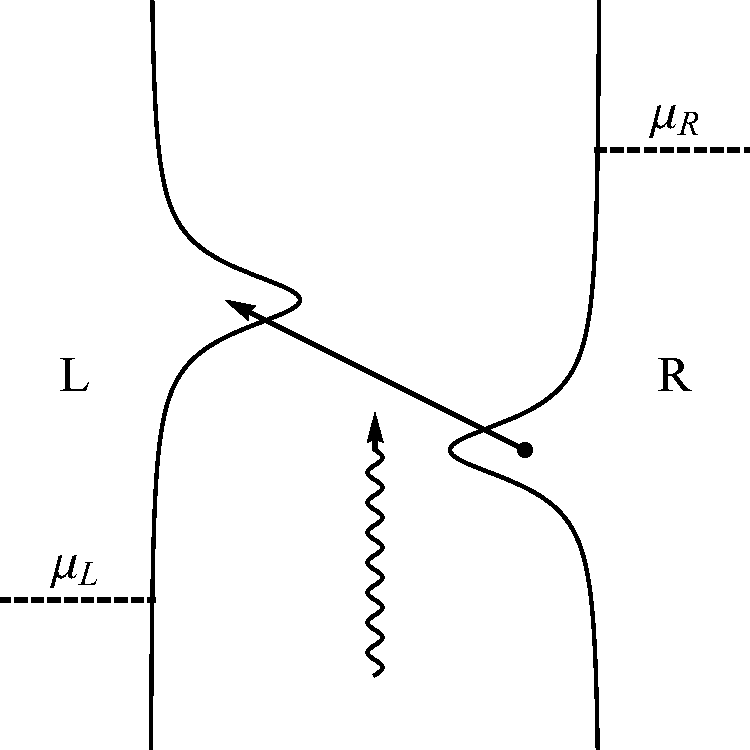
\includegraphics[width=0.2\textwidth,angle=0]{figures/fig_2b.pdf}
	}
	\caption{Two limiting cases of nonequilibrium reservoir engineering. In (a), we have a filled electronic level $\varepsilon_L$ that couples to the left electrode with chemical potential $\mu_L$, and an empty level $\varepsilon_R$ that couples to the right electrode with chemical potential $\mu_R$. We have $\mu_L>\mu_R$. Heating of the bosonic mode is due to resonant recombination of inter-electrode EHPs (process 4 in Fig.~\ref{fig:ehp}). In (b), the situation is reversed. The left state $\varepsilon_L$ is empty, while the right state $\varepsilon_R$ is filled. When $\mu_R>\mu_L$, the e-bath can be used to cool the bosonic mode through creation of inter-electrode EHPs (process $4'$ in Fig.~\ref{fig:ehp}). }
	\label{fig:resonant}
\end{figure}

In the following we show several applications of this central result.
To be more specific, we consider a minimum model of the e-bath shown in Fig.~\ref{fig:resonant}. We have two electronic states $1$ and $2$ (on-site energies $\varepsilon_1$ and $\varepsilon_2$) couple to the electrodes $L$ and $R$ with coupling parameter $\gamma_1$ and $\gamma_2$, respectively. 
Electron hopping between the two states is assisted by one bosonic mode, which at the same time couples to a ph-bath with coupling constant $\gamma_{ph}$.

\section{Applications}
%\emph{Non-reciprocal heat transport.--}
\subsection{Non-reciprocal heat transport}
Firstly, we consider the situation where the e-bath and ph-bath are in their own thermal equilibrium at two different temperature $T_e$ and $T_{ph}$. This indicates that  $\mu_{L}=\mu_{R}$ and $T_{L}=T_R=T_e$. 
If we ignore the energy dependence of $A$ in Eq.~(\ref{eq:gamma}),
$\Lambda_{mn}(\omega)=\hbar\omega{\rm tr}[M^m A M^n A]$
with $A=A_L+A_R$. Consequently,  the transmission $\mathcal{T}={\rm Tr}[\Lambda\mathcal{A}_{ph}]$ does not depend on $T_e$. Equation~(\ref{eq:jjtrans}) reduces to the Landauer formula for heat transport between two harmonic thermal baths. Thus, the EHPs behave as linear harmonic oscillator thermal baths. 


\begin{figure}[]
	% 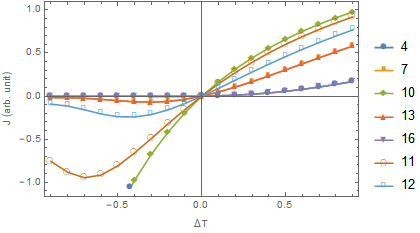
\includegraphics[scale=0.6,angle=0]{JT.png}
	% 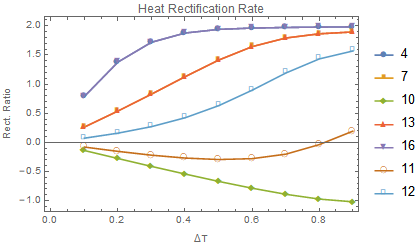
\includegraphics[scale=0.6,angle=0]{RR.png}
	%\subfigure[]{
	    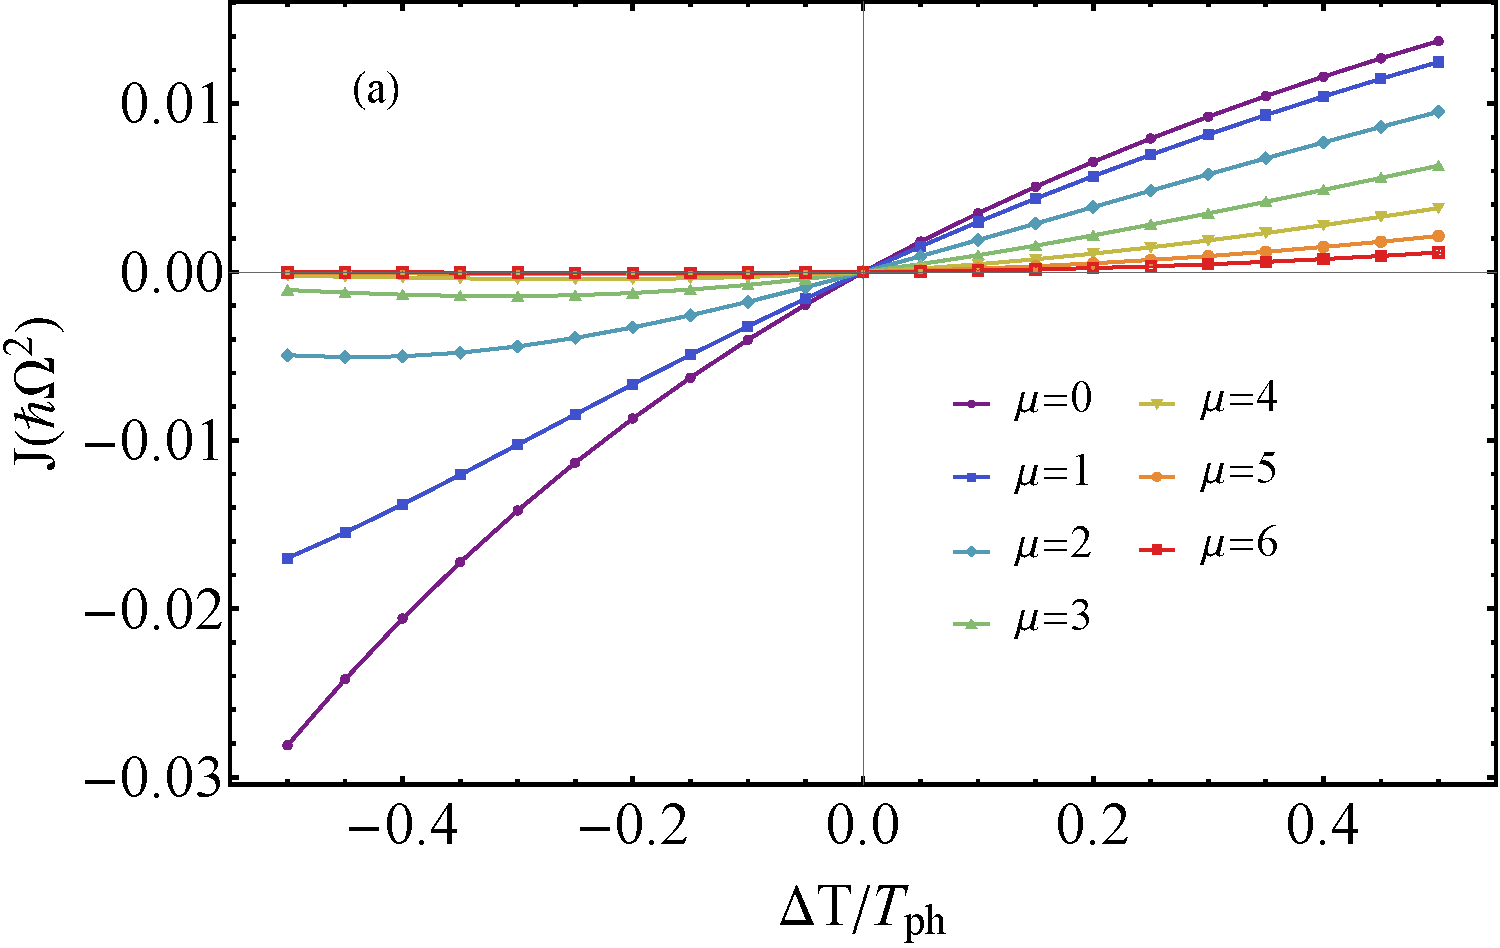
\includegraphics[width=0.45\textwidth,angle=0]{figures-0317/fig_3a.pdf}
	%}
	%\quad
	%\subfigure[]{
	    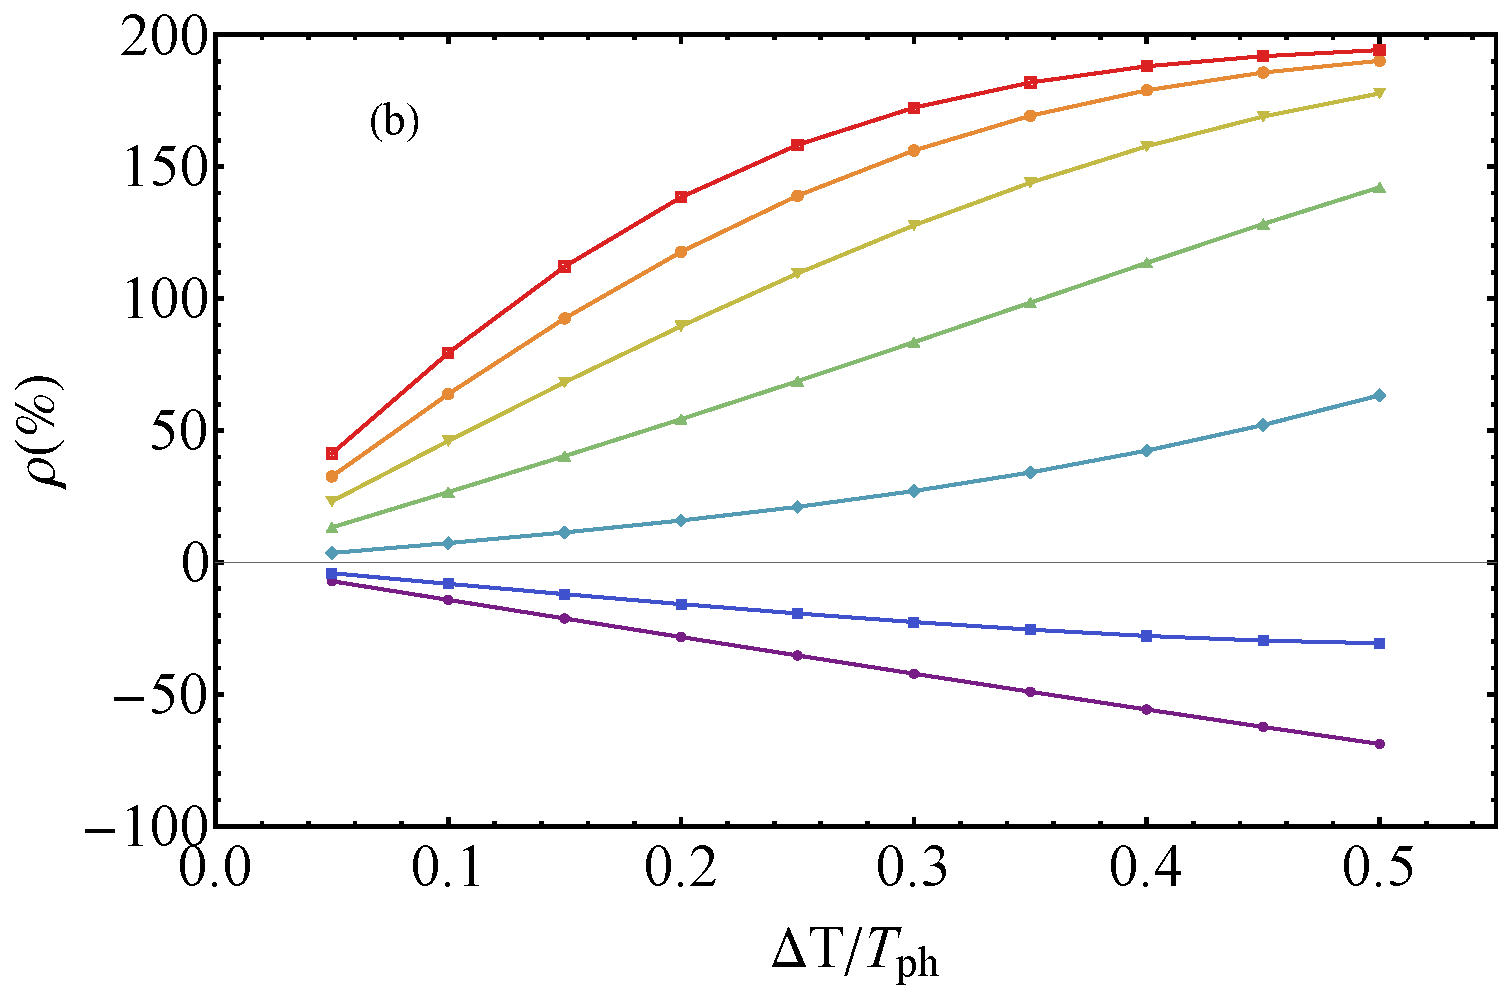
\includegraphics[width=0.44\textwidth,angle=0]{figures-0317/fig_3b.pdf}	
	%}
	\caption{Non-reciprocal heat transport in a  double dot junction shown in Fig.~\ref{fig:resonant} (a). (a) Heat current as a function of temperature difference $\Delta T/T_{\rm ph}$ for different chemical potentials. (b) Rectification ratio $\rho=(|J(|\Delta T|)|-|J(-|\Delta T|)|)/(|J(|\Delta T|)|+|J(-|\Delta T|)|)/2$ as a function of $\Delta T/T_{\rm ph}$ for different chemical potentials. We consider only one bosonic mode, whose energy is taken as unit energy. The following parameters are used in the calculation: $\varepsilon_L=0.5$, $\varepsilon_R=-0.5$, $\gamma_L=\gamma_R=0.5,m=0.5$, $\hbar\Omega=1$, $k_B=1$. }
	\label{fig:JT}
	% \revision{BZH: (1)Please shift the absolute energy such that $\varepsilon_L=-\varepsilon_R$. (2) Please mark the positions of $\mu$ in Fig. 2(a)  with short lines using the same color coding. (3) Narrow down the $x$ axis to [-0.5,0.5]. Same for Fig. 4. (1)(2)finished.}
\end{figure}

On the other hand, if we consider the energy dependence of $A(\varepsilon)$, $\Gamma(\omega)$, $\mathcal{T}^{}$ will depend on $T_e$. Energy transport becomes anharmonic. In this case, non-reciprocal energy flow is possible, i.e., $J(\Delta T)\neq J(-\Delta T)$, with $\Delta T=T_e-T_{ph}$. We thus find a necessary condition for non-reciprocal energy transport in a hybrid electron-boson system: the electron DOS in the thermal window near the chemical potential has to be energy dependent\cite{zhang2013thermal,ren2013heat}. For normal metal electrode, the energy scale of electrons is much larger than the thermal energy, leading to a flat DOS. The energy dependence of $A(\varepsilon)$ can be engineered by changing the electronic states of the central part. For example, discrete energy levels of a molecular junction or quantum dot can be used.
In Fig.~\ref{fig:JT} we have considered a two-dot junction shown in Fig.~\ref{fig:resonant} (a). We set $\mu_L=\mu_R=\mu$ and $T_e \neq T_{ph}$ to consider heat transport. The electronic DOS shows an energy dependent Lorentzian shape. This gives rise to non-reciprocal heat transport between e-bath and ph-bath. 

 %\revision{Figure~\ref{fig:resonant} shows two limiting cases. We have two electronic levels which couple to the left and right electrodes, respectively. The left level lies below $\mu_L$ is a $n$ state and the right level lies above $\mu_R$ is a $p$ state. Depending on their relative position, one of the inter-electrode EHPs couples strongest to the bosonic system. This setup has been studied in Ref.~\onlinecite{lu2011laserlike}.}







\begin{figure}[h]
	% 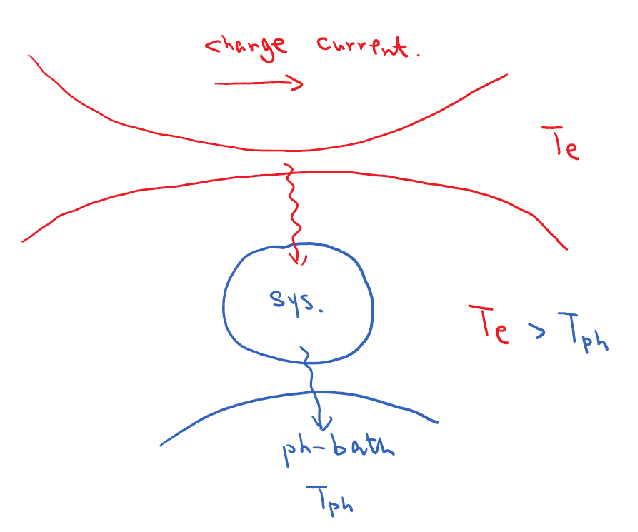
\includegraphics[scale=0.6,angle=0]{coldspot-v2.pdf}
	% 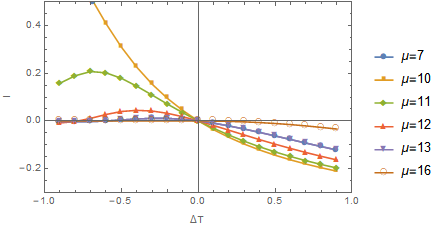
\includegraphics[scale=0.6,angle=0]{IT.png}


	%\subfigure[]{
	    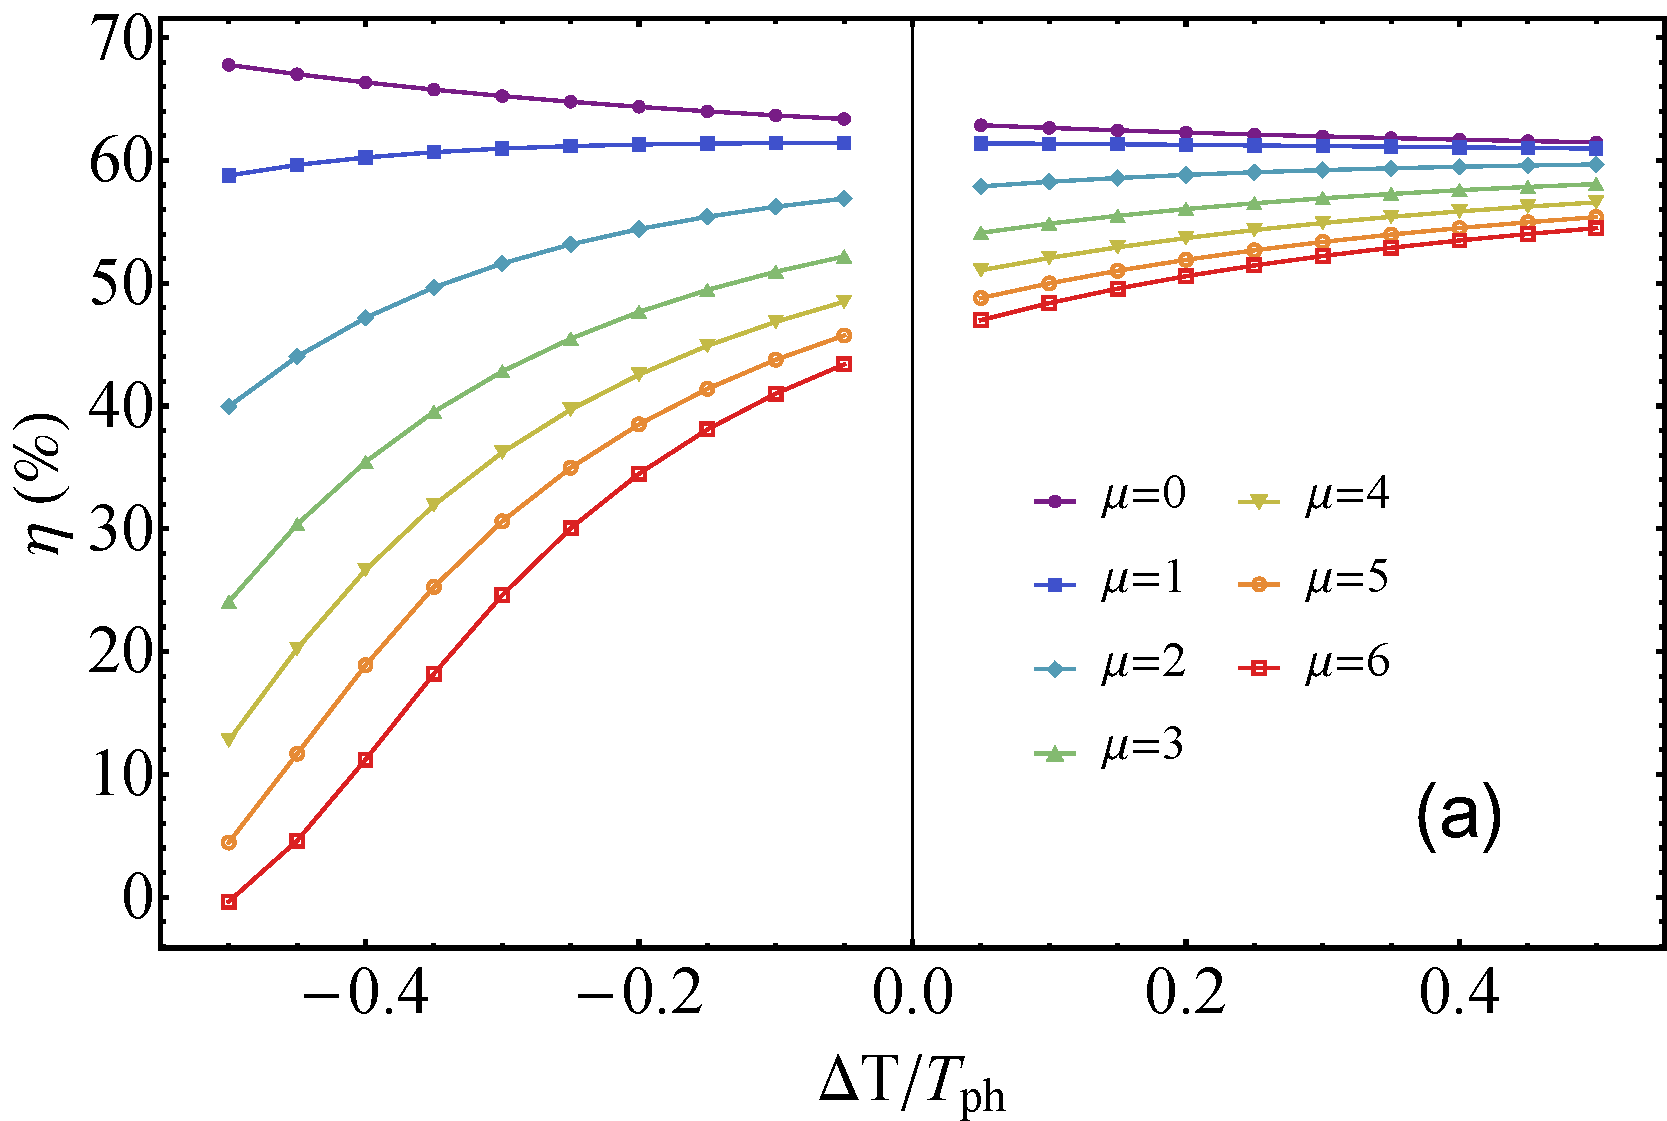
\includegraphics[width=0.45\textwidth,angle=0]{figures-0317/fig_4a.pdf}
	%}
	%\quad
	%\subfigure[]{
	    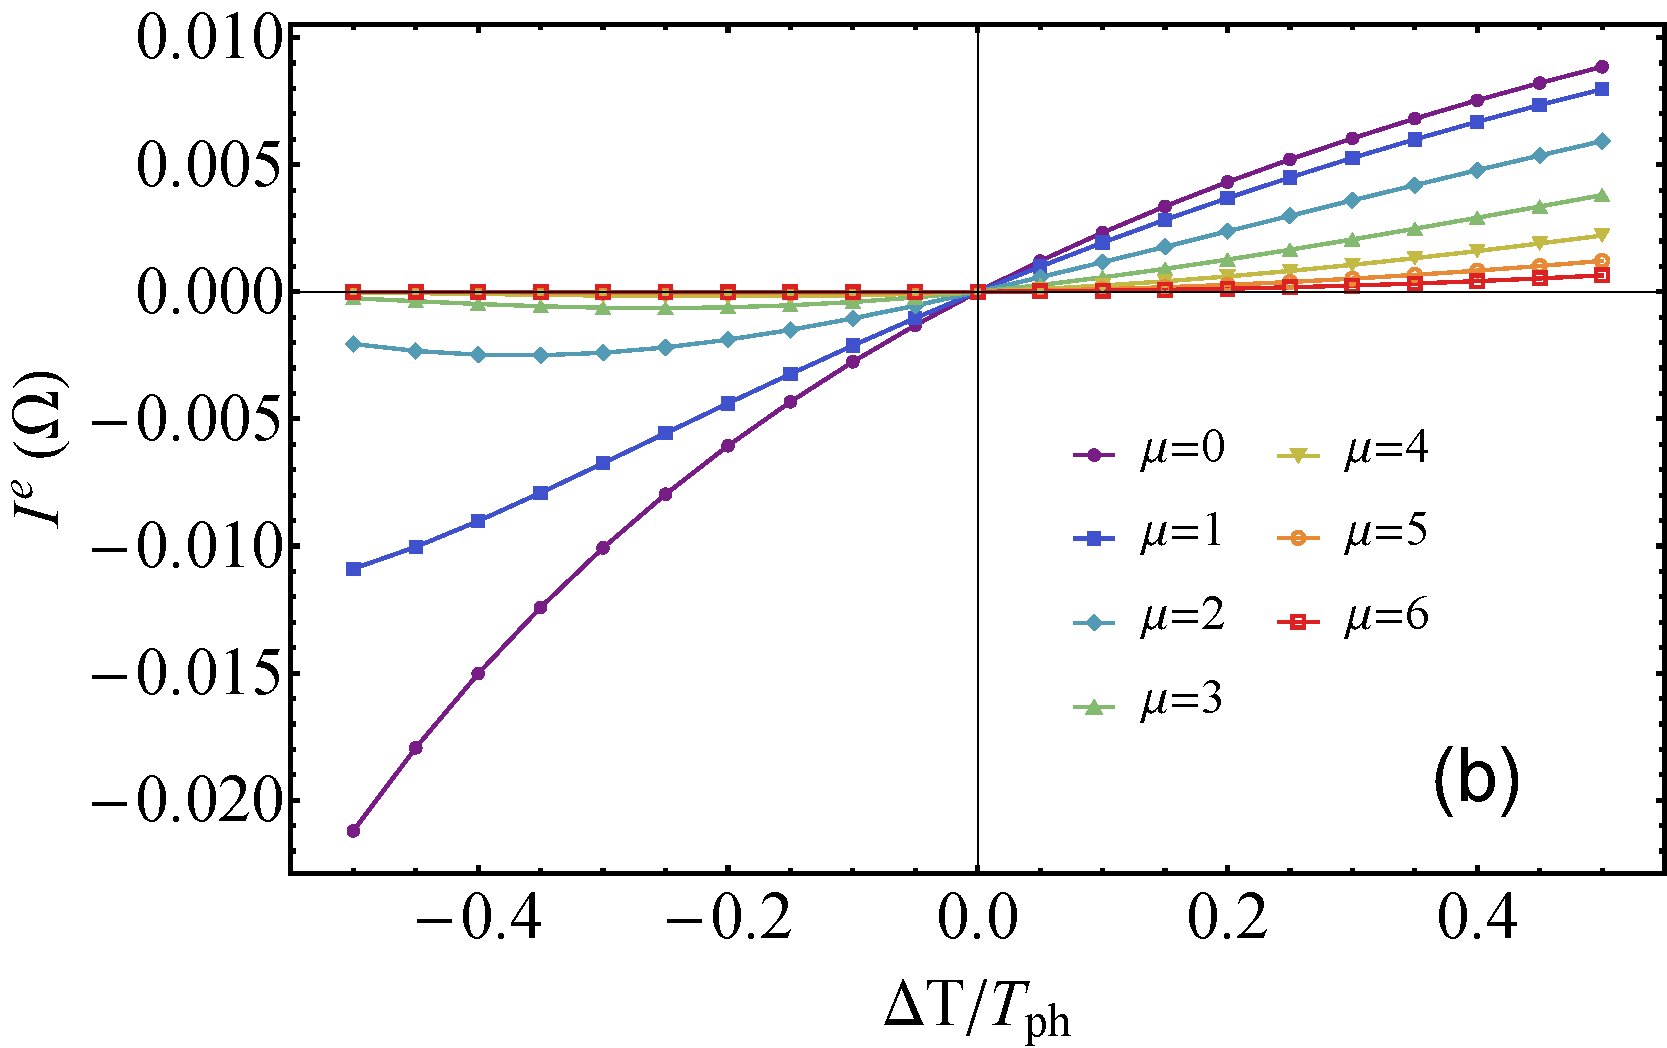
\includegraphics[width=0.48\textwidth,angle=0]{figures-0317/fig_4b.pdf}	
	%}
	\caption{Thermoelectric efficiency $\eta$ (a)  and electron particle flux $I^e$ (b) as a function of temperature difference between e-bath and ph-bath $\Delta T/T_{ph}$. The parameters are the same as Fig.~\ref{fig:JT}.   }
	\label{fig:coldspot}
\end{figure}


%\emph{ Electrical current from a cold-spot.--}
% \subsection{Hybrid thermoelectric transport}
% We can also study the thermoelectric transport of the temperature-biased electron-boson junction. When $T_{ph}\neq T_e$, in addition to the heat transport between system and e-bath, an electrical current may also be induced between the two electrodes\cite{entinwuhlman2010three,sanchez2011optimal}. In our EHP picture, this is realized through coupling of the bosonic mode with two inter-electrode EHPs. Since they contribute to two electrical current with opposite directions, in order to get a non-zero electrical current, these two channels should not get canceled. The resonant situation in Fig.~\ref{fig:resonant} can be used to enhance one of the two channels. In Fig.~\ref{fig:coldspot}, we show the thermoelectric current induced by the temperature different $\Delta T$ for different chemical potentials $\mu_L=\mu_R$ in the case of Fig.~\ref{fig:resonant} (a). The current is the largest when the chemical potential is in between $\varepsilon_L$ and $\varepsilon_R$, where the resonant enhancement is the most prominent.

% Previously, electrical current generated from a phonon hot-spot ($T_{ph}>T_e$) has been considered\cite{entinwuhlman2010three}. Our results show that the opposite is also possible, where electricity is generated by cooling the ph-bath. This demonstrates the decoupling of heat and charge transport as an advantage of thermoelectricity in hybrid nano-junctions.


\subsection{Hybrid thermoelectric transport}
 We can also study the thermoelectric transport of the temperature-biased electron-boson junction. When $T_{ph}\neq T_e$, in addition to the heat transport between system and e-bath, an electrical current may also be induced between the two electrodes\cite{entinwuhlman2010three,sanchez2011optimal}. In our EHP picture, this is realized through coupling of the bosonic mode with two inter-electrode EHPs. Since they contribute to the electrical current with opposite directions, in order to get a non-zero electrical current, these two channels should not get canceled. We can write the electron particle flux as
 \begin{align}
 I^e &= \sum_{\alpha,\beta} (\delta_{\alpha L}\delta_{\beta R} - \delta_{\alpha R}\delta_{\beta L})   \int_0^{+\infty}\frac{d\omega}{2\pi}\ {\rm Tr}[\Lambda^{\alpha\beta}(\omega)\mathcal{A}_{ph}(\omega)]\nonumber\\
 &\times [n_B(\omega-\mu_{\alpha\beta},{T}_{e})-n_B(\omega,T_{ph})].
 \label{eq:ietrans}
 \end{align}
 Here, $\delta_{\alpha/\beta, L/R}$  are the Kronecker delta functions. For simplicity, we introduce thermoelectric efficiency $\eta$ as the ratio between electron particle flux and phonon particle flux $\eta= I^e / (J^{ph}/\hbar\Omega)$.

% Obviously, all 4 EHP baths contribute phonon particle flux
% \begin{align}
% I^{ph} &= I^{ph}_{LL} + I^{ph}_{LR} + I^{ph}_{RL} + I^{ph}_{RR}.
% \label{eq:iph}
% \end{align}

% Here, $I^{ph}_{\alpha\beta}$ is the phonon particle flux contribution of EHP bath $\alpha\beta$

% \begin{align}
% I^{ph}_{\alpha\beta} &= \int_0^{+\infty}\frac{d\omega}{2\pi}\ {\rm Tr}[\Lambda^{\alpha\beta}(\omega)\mathcal{A}_{ph}(\omega)]\nonumber\\
% &\times [n_B(\omega-\mu_{\alpha\beta},{T}_{e})-n_B(\omega,T_{ph})].
% \label{eq:iphab}
% \end{align}

% On the other hand, only LR and RL baths contribute electron particle flux. Further more, according to EHP reaction equation equation (\ref{eq:reaction}) and equation (\ref{eq:reaction2}), 
% \begin{align}
% I^e_{LR}=I^{ph}_{LR},~I^e_{RL}=-I^{ph}_{RL}. 
% \label{eq:ie}
% \end{align}


% Thus, electron particle flux can be expressed by phonon particle flux contribution
% \begin{align}
% I^{e} =I^{e}_{LR} + I^{e}_{RL} = I^{ph}_{LR} - I^{ph}_{RL}.
% \label{eq:ie}
% \end{align}

% Finally, our thermoelectric current generation efficiency 
% \begin{align}
% \eta = \frac{I^{ph}_{LR} - I^{ph}_{RL}}{I^{ph}_{LL} + I^{ph}_{LR} + I^{ph}_{RL} + I^{ph}_{RR}}.
% \label{eq:tcge}
% \end{align}


 The resonant situation in Fig.~\ref{fig:resonant} can be used to enhance one of the two channels. In Fig.~\ref{fig:coldspot} (b), we show the thermoelectric current induced by the temperature different $\Delta T$ for different chemical potentials $\mu_L=\mu_R$ in the case of Fig.~\ref{fig:resonant} (a). The efficiency $\eta$ in Fig.~\ref{fig:coldspot} (a) is the largest when the chemical potential is in between $\varepsilon_L$ and $\varepsilon_R$, where the resonant enhancement is the most prominent.
 Previously, electrical current generated from a phonon hot-spot ($T_{ph}>T_e$) has been considered\cite{entinwuhlman2010three}. Our results show that the opposite ($T_{ph}<T_e$) is also possible, where electricity is generated by cooling the ph-bath. This demonstrates the decoupling of heat and charge transport as an advantage of thermoelectricity in hybrid nano-junctions.

%Notably, when $T_{ph}<T_{e}$ and $\mu_L=\mu_R$. The temperature difference between e-bath and ph-bath generates a heat current flow from the e-bath to the ph-bath. At a result of the heat transport, electron transport between $L$ and $R$ electrode takes place.

%\emph{Electronic cooling of bosonic mode.--}
\subsection{Electronic cooling of bosonic mode}
We now turn on the voltage bias in the e-bath.
The applied voltage changes the initial and final electron states of the EHP excitation. Thus, the EHP DOS can be modified by voltage. More importantly, the inter-electrode EHPs acquire a non-zero chemical potential, EHP-4 has a chemical potential of $\mu_{LR}$, while EHP-3 gets a chemical potential with opposite value $\mu_{RL}$. 
\begin{figure}[h]
	% 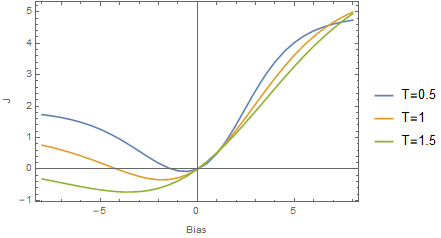
\includegraphics[scale=0.55,angle=0]{Cooling.png}
	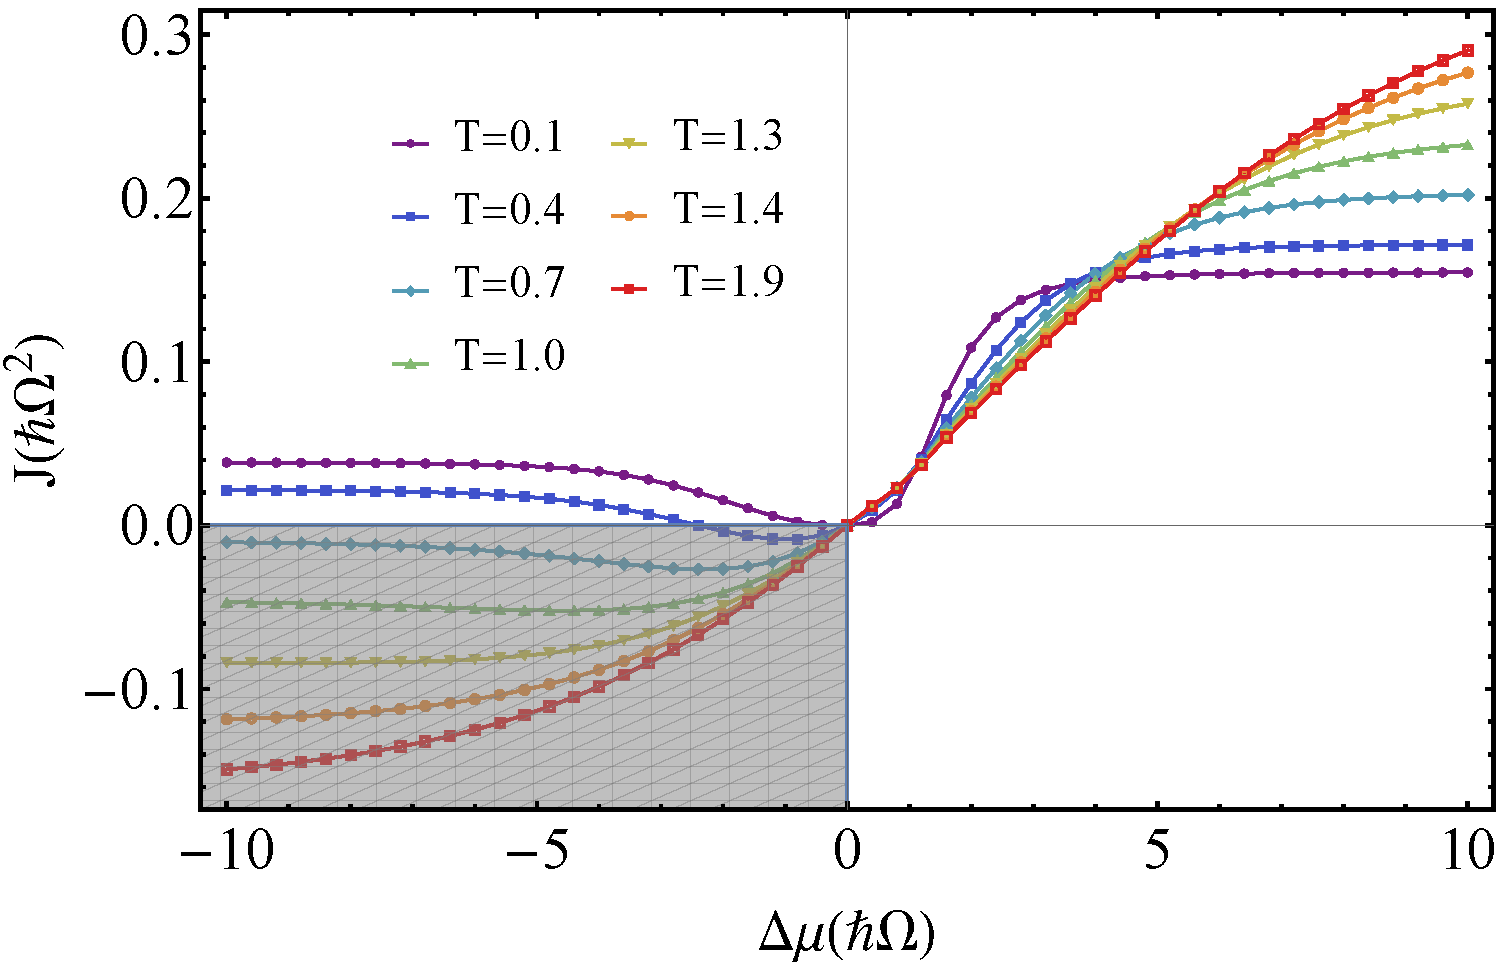
\includegraphics[width=0.5\textwidth,angle=0]{figures/fig_5.pdf}	
	\caption{Energy current $J$ from the e-bath to the bosonic mode as a function of chemical potential $\mu_{LR}$, corresponding to the situation in Fig.~\ref{fig:resonant} (b). Negative $J$ (gray shaded area) means cooling of the bosonic mode.  }
	\label{fig:cooling}
\end{figure}
Change of the chemical potential breaks the equilibrium in the reaction, and drives the energy transport between e-bath and the system. 
Direction of energy flow depends on the relative magnitude of two fluxes. It can be engineered by tuning the electronic band structure, or more specifically, the transition probability of the two types of EHP excitation. 

In the case shown in Fig.~\ref{fig:resonant} (b), process $4'$ is resonantly enhanced. Electronic cooling becomes possible using this resonant enhancement. This is demonstrated in Fig.~\ref{fig:cooling}, where the heat current from the e-bath to the system $J$ is plotted as a function of voltage bias $\mu_{LR}$ while keeping temperature fixed $T_e=T_{ph}=T$. For negative bias, we observe a negative $J$ regime. The range of this regime gets larger for higher temperature $T$. This is the electronic cooling of the bosonic mode. Very recently, experimental demonstration of near field radiative cooling using a reversely biased $p$-$n$ junction has been demonstrated \cite{zhu2019near}. The experimental results can be understood using this simple model.



%Joule heating in molecular conductors has been studied 

%The forward reaction $e_L+h_R \to p_n$  is enhanced, leading to energy flow from the EHPs to the bosonic mode. Meanwhile, that of $e_R+h_L \to p_n$ is reduced, leading to an opposite energy flow. Direction of the total energy current is determined by the relative magnitude of the two processes, i.e., the magnitude of the transmission $T^{\alpha\beta}$. As an illustration, we consider electronic cooling of the bosonic mode. 
%\begin{figure}[]
%	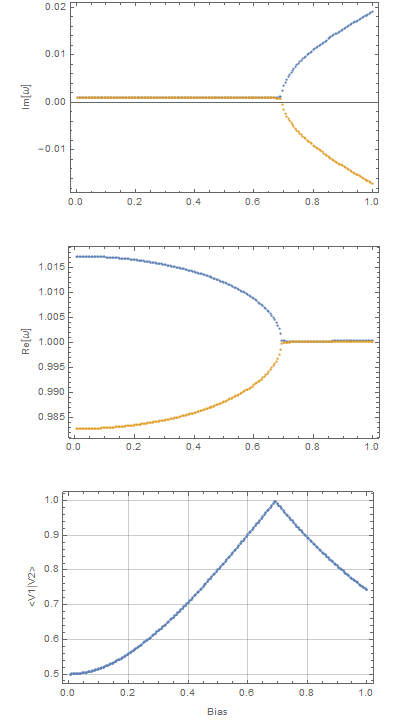
\includegraphics[scale=0.5,angle=0]{ep.png}
%	\caption{Emergence of exceptional point due to coupling to a nonequilibrium e-bath. The effective dynamical matrix is given in Eq.~(\ref{eq:kk}). The following parameters are used: $\Omega=1$, $\delta=0.04$, $\gamma=0.001$, $a=0.05$, $b=0.0$, $c=0.02$. }
%	\label{fig:ep}
%\end{figure}

%\emph{Current-induced exceptional point in two-mode system.--}
%\subsection{Current-induced exceptional point in two-mode system}
%So far, we have only considered one bosonic mode in the system. Now we show that the nonequilibrium e-bath can be used to couple two otherwise isolated bosonic modes. The bias dependence of coupling parameters can be used to tune the system to an exceptional point, where both the eigen values and eigen vectors of the two modes coalesce. 
%
%To illustrate this effect, we consider two identical bosonic modes with average frequency $\Omega$ and a small detuning $\delta$, such that $\omega_{\pm}=\Omega\pm \delta/2$. Extra damping of the two modes $\gamma_1$ and $\gamma_2$ are introduced to account for their coupling to e-bath and ph-bath. Importantly, the nonequilibrium nature of the e-bath introduces coherent coupling between the two otherwise isolated modes, which are proportional to the applied bias $V$. Putting together, we have the following effective dynamical matrix for the two modes
%\begin{equation}\label{eq:kk}
%\left[
%\begin{array}{cc}
%(\Omega+\delta/2+i \gamma)^2 & V(a+i b \Omega) + i c\Omega \\
%-V (a+i b \Omega)+i c\Omega & (\Omega-\delta/2+i \gamma)^2
%\end{array}
%\right].
%\end{equation}
%Here, $a$ and $b$ are non-zero only in the presence of voltage bias in the e-bath, which correspond to the currend-induced non-conservative and effective Lorentz force, respectively\cite{lu_blowing_2010}. Meanwhile, $c$ and $\gamma$ account for the damping due to coupling to ph-bath and/or e-bath. If we ignore the energy dependence of electron spectral function within the voltage bias window, $a={\rm Im}{\rm tr}[M^1 A_L M^2 A_R]/\pi$ becomes constant, $b=0$. This approximation is valid if the electron bandwidth $D$ is much larger than the corresponding mode energy $\hbar\Omega$, i.e., $D\gg \hbar\Omega$. Figure~\ref{fig:ep} shows a typical example for this model. We have plotted the imaginary (a), the real (b) part of the eigen values as a function of bias. The exceptional point corresponds to the place where both parts are the same for the two modes. Additionally, at this point the inner product of the two eigen vectors takes the maximum value 1, meaning that the eigen vectors coalesce.


\section{Conclusions}
In summary, we have shown that a normal two-probe electron conductor can be effectively viewed as EHP baths with chemical potential determined by the applied voltage bias. This is made possible by introducing the inter-electrode charge transfer EHPs. Properties of the EHP baths can be engineered through tuning the parameters of the conductor and the external voltage bias. This bath engineering provides an efficient way of controlling hybrid energy and thermoelectric transport in electron-boson junctions. 

% \revision{BZH: Please check the references and use abbreviations for all the journal names.}

\begin{acknowledgements}
The authors thank J.-S. Wang and M. Brandbyge for discussions. This work is supported by the National Natural Science Foundation of China
(Grant No. 21873033), the National Key Research and Development Program of China
(Grant No. 2017YFA0403501) and the program for HUST academic frontier youth team.
\end{acknowledgements}
%%%%%%%%%%%%%%%%%%%%%%%%%%%%%%%%%%%%%%%%%%%%%%%%%%%%5
\if false
\clearpage
\appendix
\section{introduction}
How to understand the transport phenomena in microscopic systems (such as quantum dots or wires, molecules, graphene, etc.) is a key problem. A series of
theories have been developed to explain them, in which the scattering approach by Landauer\cite{landauer1957spatial} and B\"{u}ttiker\cite{buttiker1986four} is the most commonly used, termed Landauer formalism. The initial application of this formula is the noninteracting electrons, hereafter, which was extended to include the electron-Boson and electron-electron interactions\cite{meir1992landauer,jauho1994time,lu2007coupled}.
In the Landauer formalism, the current through a two or multi- terminal device (including electrodes and a finite region) can be expressed generally by the transmission coefficient and distributions of the electrodes. This has been utilized in areas ranging from molecular electronics, spintronics to optoelectronics\cite{galperin2007molecular,haug2008quantum,galperin2012molecular}.

%One may ask a question: \emph{Is there a formula similar to Landauer in the Bose system}? 
On the other hand, the Landauer-like formula for Bose system has been proposed, in which the current is driven by the temperature bias between two heat baths\cite{wang2006nonequilibrium,wang2007nonequilibrium,wang2008quantum,ojanen2008mesoscopic,ruokola2009thermal,li2012colloquium,taylor2015quantum,wang2016landauer}. One may ask a question: \emph{Can the current be driven by an effective chemical potential of Boson}? To answer this question, we may propose a phenomenological Landauer-like formula 
\begin{equation}
\begin{split}
J_{B}=\int_{-\infty}^{+\infty}\hbar\omega \tau(\omega)[n_{L}(\omega,\nu_{L},T_{L})-n_{R}(\omega,\nu_{R},T_{R})],
\end{split}
\label{Bose-LB}
\end{equation}
where $\tau(\omega)$ is the transmission coefficient, $n_{\alpha}(\omega,\nu_{\alpha},T_{\alpha})=[e^{(\hbar\omega-\nu_{\alpha})/k_{B}T_{\alpha}}-1]^{-1}$ is the Bose-Einstein
distribution function in bath $\alpha=L/R$ with the effective chemical potential $\nu_{L/R}$ and the temperature $T_{L/R}$. 
%In fact, the LB-like formula for thermoradiative from a biased semiconductor has been proposed. 
To date, the importance of Eq.~(\ref{Bose-LB}) has not been clarified in the quantum transport, especially in systems with electron-Boson interactions, such as electron-phonon and electron-photon.

In this paper, we will try to demonstrate that Eq.~(\ref{Bose-LB}) for the energy transport through coupled electron-Boson system is highly desirable. We first propose an effective model and Hamiltonian that can describe the Eq.~(\ref{Bose-LB}). Three examples in order to clarify the Eq.~(\ref{Bose-LB}) will be discussed: heat transport through a coupled electron-phonon system, light emission from single molecules, and near field thermal radiation.
Moreover, the application of Eq.~(\ref{Bose-LB}) will be presented.

\section{Model}
We cosider a Bose system coupled to two heat baths, as shown in Fig.~\ref{Fig01}. The corresponding Hamiltonian takes the form
\begin{equation}
\begin{split}
H=H_{L}+H_{B}+H_{R}+H_{LB}+H_{BR},
\end{split}
\label{hamiltonian}
\end{equation}
%L可以是一个有效的,非平衡的
%中间区域要看定义
%右边可以是一个平衡的库
%以下三个例子只需要改变左边的非平衡的hamiltonian
where $H_{L}$ describes the left bath. It can be regarded as an effective nonequilibrium bath driven by a bias voltage, such that $T_{L}>0$ and $\nu_{R}\neq0$. $H_{R}$ represents a equilibrium (nonequilibrium) bath with $T_{R}>0$ and $\nu_{R}=0$ ($\nu_{R}\neq0$). $H_{B}$ is the Bose system, which can be viewed as the scattering center. $H_{LB}$ and $H_{BR}$ represent the system-bath couplings.

In the following, we will present that the coupled electron-Boson system can be described by the effective model in Fig.~\ref{Fig01}. Specifically, the non-zero Bose chemical potential is driven by electron system with electron-Boson coupling under a bias voltage. Meanwhile, the energy transport in such systems is naturally carried out by Eq.~(\ref{Bose-LB}).
%
\begin{figure}[h]
\centering
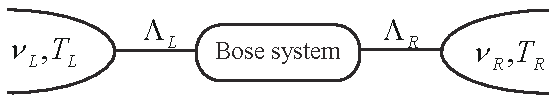
\includegraphics[width=8 cm]{photon-Landauer.pdf}
\caption{ Schematic view of a Bose system connected to two Bose baths. $T_{L,R}$, $\nu_{L,R}$, and $\Lambda_{L/R}$ are the temperature, the chemical potential, and the coupling bewteen system and heat bath.}
\label{Fig01}
\end{figure}
%


\section{Examples}
\subsection{Heat transport through a coupled electron-phonon system}
Without loss of generality, we consider a four terminal coupled electron-phonon model, as illustrated
in Fig.~\ref{heat}.
%
\begin{figure}
\centering
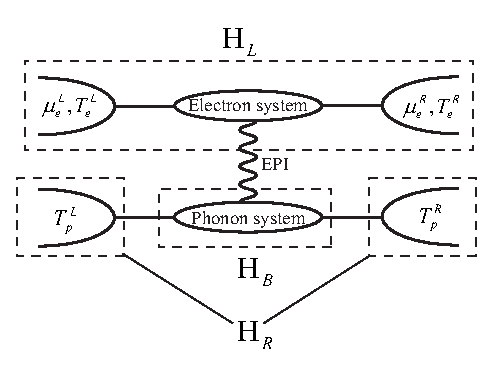
\includegraphics[width=8 cm]{heat.eps}
\caption{A four terminal coupled electron-phonon system, in which the electron and phonon subsystem are connected by electron-phonon interaction (EPI) .}
\label{heat}
\end{figure}
%
There is a finite voltage bias between two electron bath, i.e., $\mu_{e}^{L}=eV/2$, $\mu_{e}^{R}=-eV/2$, and $T_{e}^{L}=T_{e}^{R}=T_{p}^{L}=T_{p}^{R}$. In this case, the Joule heating driven by electron-phonon interaction becomes important. By means of the nonequilibrium Green’s function (NEGF) method, the energy transfer from electron to phonon system can be written as\cite{lu2007coupled}
\begin{equation}
\begin{split}
Q=-i\int\frac{d \varepsilon}{2 \pi}\int\frac{d \omega}{2 \pi}\hbar\omega{\rm Tr}[{\rm tr}[MG_{0}^{>}(\varepsilon)M
G_{0}^{<}(\varepsilon-\hbar\omega)]D_{0}^{<}(\omega)].
\end{split}
\end{equation}
Here, $G_{0}$ and $D_{0}$ are the bare Green functions of electronic and phononic degrees of freedom, $M$ is electron-phonon coupling matrix. 
By introducing the DOS and the time-reversed DOS of electrons and phonons induced by electrode $\alpha(=L,R)$\cite{lu2016electron}
\begin{equation}
\begin{split}
&A_{\alpha}(\varepsilon)=G_{0}^{r}(\varepsilon)\Gamma_{\alpha}^{e}(\varepsilon)G_{0}^{a}(\varepsilon),\\
&\tilde{A}_{\alpha}(\varepsilon)=G_{0}^{a}(\varepsilon)\Gamma_{\alpha}^{e}(\varepsilon)G_{0}^{r}(\varepsilon),\\
&A(\varepsilon)=A_{L}(\varepsilon)+A_{R}(\varepsilon),
\end{split}
\end{equation}
and
\begin{equation}
\begin{split}
&\mathcal{A}_{\alpha}(\omega)=D_{0}^{r}(\omega)\Gamma_{\alpha}^{p}(\omega)D_{0}^{a}(\omega),\\
&\mathcal{\tilde{A}}_{\alpha}(\omega)=D_{0}^{a}(\omega)\Gamma_{\alpha}^{p}(\omega)D_{0}^{r}(\omega),\\
&\mathcal{A}(\omega)=\mathcal{A}_{L}(\omega)+\mathcal{A}_{R}(\omega).
\end{split}
\end{equation}
The energy flux can be written as (see Appendix \ref{L-phonon} for details)
\begin{equation}
\begin{split}
Q&=\int\frac{d \omega}{2 \pi}\hbar\omega{\rm Tr}[\Lambda_{LR}\mathcal{A}(\omega)][n_{B}(\hbar\omega;T_{p})-n_{B}(\hbar\omega-eV;T_{e})],
\end{split}
\label{Landauer-phonon}
\end{equation}
where $T_{p}=T_{p}^{L}=T_{p}^{R}$ and $T_{e}=T_{e}^{L}=T_{e}^{R}$. Eq.~\ref{Landauer-phonon} is a phononic analog to the Landauer transport formula in nonequilibrium state, in which the driven bias is the effective chemical potential ${\rm eV}$ of Bosons. In fact, the nonequilibrium electron subsystem with electron-phonon coupling modelled by $H_{L}$ in Fig.~\ref{heat} satisfies a Bose distribution with an effective chemical potential, which can be obtained by means of rate equation\cite{lu2011laserlike}. 
% The population of current-induced excitation of a certain phonon is
%\begin{equation}
%\begin{split}
%\frac{d}{dt}N_{p}=\mathbb{E}(N_{p}+1)-\mathbb{A}N_{p},
%\end{split}
%\label{rate-equation}
%\end{equation}
%where $\mathbb{E}$ and $\mathbb{A}$ corresponding to emission and absorption processes, respectively. 
%The rates can be calculated by using Fermi's golden rule 
%\begin{equation}
%\begin{split}
%\mathbb{E}&=\frac{2\pi}{\hbar}\sum_{if}\mid\langle \Psi_{f}\mid H_{LB}\mid %\Psi_{i}\rangle\mid^{2}F_{i}(1-F_{f})\delta(\varepsilon_{f}-\varepsilon_{i}+\hbar\Omega),\\
%\mathbb{A}&=\frac{2\pi}{\hbar}\sum_{if}\mid\langle \Psi_{f}\mid H_{LB}\mid %\Psi_{i}\rangle\mid^{2}F_{f}(1-F_{i})\delta(\varepsilon_{f}-\varepsilon_{i}-\hbar\Omega),
%\end{split}
%\end{equation}
%In steady state (ss), $\frac{d}{dt}N_{p}=0$, we can get (see Appendix \ref{phonon-distribution} for %details)
%\begin{equation}
%\begin{split}
%N_{ss}=\frac{1}{(\mathbb{A}/\mathbb{E})-1}=\frac{1}{e^{(\mu_{fi}-\hbar\Omega)/k_{B}T}-1}.
%\end{split}
%\label{phonon-SS}
%\end{equation}

%Under this framework, the energy transport in all systems with electron-phonon coupling can be described by the Landauer-type formula. The following issues can be addressed


%%%%%%%%%%%%%%%%%%%%%%%%%%%%%%%%%%%%%%%%%%%%%%%%%%%%%%%%%%%%%%%%%%%%%%%%%%%%%%%%%%%%%%%
\subsection{Light emission from single molecules}
%
\begin{figure}[h]
\centering
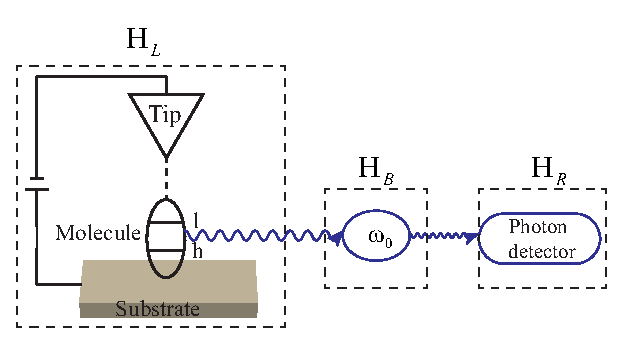
\includegraphics[width=8 cm]{STM-light-emission.eps}
\caption{ STM-induced light emission from a single molecule.}
\label{STM-emission}
\end{figure}
%
In scanning tunneling microscope (STM) induced single molecule electroluminescence experiments, the light emission induced by the recombination of electrons and holes injected from STM tip and substrate has been clarified by experiment and theory\cite{qiu2003vibrationally,tian2011density,zhu2013self,reecht2014electroluminescence,bergfield2018signatures}. Specifically, when a voltage bias exists between Tip and substrate, an electron and a hole will tunnel to LUMO (l) and HOMO (h) levels from Tip and substrate (see Fig.~\ref{STM-emission}), such that the light emission excited by the recombination of them can be observed. Because this is no coupling between LUMO and HOMO, the energy of electrons (holes) is approximately equal to the chemical potential of Tip (substrate), that is, $\varepsilon_{l}=\mu_{t}$ and $\varepsilon_{h}=\mu_{s}$.

The process of light emission in Fig.~\ref{STM-emission} is similar to the chemical reaction, that is, the recombination of an electron (e) and a hole (h) produces a photon (p)
\begin{equation}
\begin{split}
e+h\rightleftharpoons p.
\end{split}
\end{equation}
For the minimum of the free energy, we can get
\begin{equation}
\begin{split}
dE=\mu_{e}dn_{e}+\mu_{h}dn_{h}+\mu_{p}dn_{p}=0.
\end{split}
\end{equation}
where $n_{e,h,p}$ is the particle numbers of electron/hole/photon.
The conservation of particle numbers requires 
\begin{equation}
\begin{split}
dn_{e}=dn_{h}=-dn_{p}.
\end{split}
\end{equation}
Finally, we have
\begin{equation}
\begin{split}
\mu_{e}+\mu_{h}=\mu_{p},
\end{split}
\end{equation}b
where $\mu_{p}$ is the chemical potential of photon. The sum $\mu_{e}+\mu_{h}$ is the difference $\varepsilon_{e}-\varepsilon_{h}$ of the quasi-Fermi energies of the electrons in the LUMO band and
holes in the HOMO, respectively\cite{wurfel1982chemical}. For our case, $\varepsilon_{e}-\varepsilon_{h}=$eV. 

Based on NEGF method and the Hamiltonian of the model in Fig.~\ref{STM-emission}(see Appendix \ref{STM-Hamiltonian}), for the energy flow from the electronic system to the photonic system, we can get a Landauer-type formula similar to Eq.~\ref{Landauer-phonon}. The energy-dependent flux can be defined to study the light emission from a molecule-mediated STM juction\cite{nian2018fano}.

%\begin{equation}
%\begin{split}
%Q&=\int\frac{d \omega}{2 \pi}\hbar\omega{\rm %Tr}[\Lambda_{LR}\mathcal{A}(\omega)][n_{B}(\hbar\omega;T)-n_{B}(\hbar\omega-eV;T)].
%\end{split}
%\label{Landauer-phonon}
%\end{equation}
%This is similar to an coupled electron-phonon system. The energy-dependent flux can be defined as
%\begin{equation}
%\begin{split}
%Q_{0}(\omega)d\omega&=\frac{\hbar \omega}{2 \pi}{\rm %Tr}[\Lambda_{LR}\mathcal{A}(\omega)][n_{B}(\hbar\omega;T)-n_{B}(\hbar\omega-eV;T)]d\omega.
%\end{split}
%\label{Landauer-phonon}
%\end{equation}
%The light emission from a single molecule driven by a STM tip can be simulated by the above formula. 


\subsection{Radiative heat transfer}
%In general, the thermal radiation takes place when two bodies have different temperatures and zero chemical potentials. The power exchanged between the two bodies can be calculted by the Landauer-like formula in Eq.~\ref{Bose-LB} by setting $\nu_{L}=\nu_{R}=0$ and $T_{L}\neq T_{R}$\cite{biehs2011nanoscale,moncada2015magnetic,ben2016photon,zhu2016persistent,latella2017giant,zhu2018theory,ben2019thermal}. Recently, Fan's group proposed a new thermal radiation device\cite{chen2015heat,chen2016near}, in which the semiconductor p−n junction under an external bias as a source of thermal radiation, such that the expectation value of the photon energy per mode above the band gap satisfies the Bose distribution with nonzero chemical potential\cite{wurfel1982chemical}. Then the thermal radiation can be transferred from the hotter body to the colder body with zero chemical potential. 
%
\begin{figure}
\centering
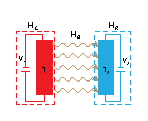
\includegraphics[width=8 cm]{radiation.eps}
\caption{ Schematic of the configuration for two-body thermal radiation. $V_{1}$ ($V_{2}$) and $T_{1}$ ($T_{2}$) represent the bias voltage and temperature of the two bodies, respectively. }
\label{thermal-radiation}
\end{figure}
%

The thermal radiation mechanism can be described by the model in Fig.~\ref{thermal-radiation} and can be projected into the general model in Fig.~\ref{Fig01}. In this case, the Eq.~\ref{Bose-LB} with $\nu_{L}\neq 0$ (and $\nu_{R}=0$) and $T_{L}=T_{R}\neq 0$ can be used to fitted the thermal radiation. What's more, we may predict another thermal radiation device consisting of two semiconductor p-n junctions at different external biases, as shown in Fig.~\ref{thermal-radiation}. The thermal radiation will be flowing from the terminal with high bias to the one with low bias. This may provide a new idea to control the derection of thermal radiation.


\section{Applications}
%\subsection{Joule heating}
%The Joule heating in such coupled electron-phonon system can be described by Eq.~(\ref{Landauer-phonon}).

%\bullet \ Phononic \ cooling

In current carrying molecular junctions, the heating induced by vibrational excitation is a common process\cite{yu2004inelastic,galperin2007molecular,huang2007local,ioffe2008detection,hartle2011vibrational,simine2012vibrational}. This occurs when the molecular levels are located in the bias window and bias voltage exceeds molecular vibrational frequencies. Once the energy dissipation from molecule junction to environment is not effective enough, the temperature of the junction will be increased, leading to its instability or even breakdown. Therefore, cooling the molecular junction is important for building molecular-based electronic devices\cite{galperin2009cooling,hartle2011resonant,hartle2018cooling}.

In Eq.~\ref{Landauer-phonon} $Q$ represents the energy transfer from electron to phonon subsystem. So, the phonon cooling occurs when $Q<0$ and $T_{e}>T_{p}$. This indicates that the energy flux can flow from phonon system with low temperature to electron system with high temperature. 

%\bullet \ Photonic \ cooling

The optical cooling of solids driven by coherent laser light has been observed\cite{epstein1995observation}. Recently, Zhu \emph{et al}. proposed a incoherent way to control the thermal radiation in a photodiode combined with an enhanced transfer of near field thermal radiation\cite{zhu2019near}. In this experiment, the authors can adjust the chemical potential of photons to achieve the near-field photonic cooling.

In general, the nonzero chemical potential can be realized in two ways\cite{herrmann2005light}: (1) The light is induced by a photochemical reaction. If the light is in chemical
equilibrium with the excitations of matter (such as single molecules) whose chemical
potential is nonzero, for example, the electron-hole pairs in STM junction; (2) Another way to obtain $\mu_{p}\neq 0$ is driven by a thermodynamic process. One can start with $\mu_{p}=0$ and change the chemical potential in a thermodynamic. Once photons do not interact with matter, a zero chemical potential can be achieved. 

Based on Eq.~\ref{Bose-LB} and the model in Fig.~\ref{thermal-radiation}, we can provide a more clearer explaination of the photonic cooling. As shown in Fig.~\ref{thermal-radiation}, the chemical potentials of the cold body 2 and the hot body 1 are set to be $V_{2}>0$ and $V_{1}=0$, then a net heat flow from the cold body to the hot one can be obtained. What's more, by setting $V_{1}<0$ and $V_{2}=0$, one can observed the negative luminescence\cite{chen2016near}, and a net heat flow from cold body 2 to the hot body 1 can also be obtained.

%\bullet \ Heat \ rectification

In this case, we set the voltage bias between two electrodes is 0, that is, $\mu_{e}^{L}=\mu_{e}^{R}$. Meanwhile, a temperature bias is presented between electron and phonon subsystem, that is, $T_{e}^{L}=T_{e}^{R}\neq T_{p}^{L}=T_{p}^{R}$. 
%Then Eq.~(\ref{Landauer-phonon}) becomes
%\begin{equation}
%\begin{split}
%Q&=\int\frac{d \omega}{2 \pi}\hbar\omega{\rm %Tr}[\Lambda_{LR}\mathcal{A}(\omega)][n_{B}(\hbar\omega;T_{p})-n_{B}(\hbar\omega;T_{e})].
%\end{split}
%\label{L-BR}
%\end{equation}

In Eq.~\ref{Landauer-phonon}, the term $[n_{B}(\hbar\omega;T_{p})-n_{B}(\hbar\omega;T_{e})]$ is temperature dependent. Then the effective transmission function ${\rm Tr}[\Lambda_{LR}\mathcal{A}(\omega)]$ is key for heat rectification. It is obviously to verify that the heat rectification vanishes when $\Lambda_{LR}$ is a constant, that is, $\Lambda_{LR}$ is temperature independent. Our analysis can be identified by examining the energy transport in metal-insulator interface with electron-phonon  scattering\cite{zhang2013thermal,ren2013heat} and insulating ferromagnetic spin junction with spin-phonon interaction\cite{zhang2017thermal}.

\section{Conclusion}

In summary, we have proposed a nonequilibrium Landauer formula and constructed a model for coupled electron-Boson systems. The Landauer approach developed here allows for analytical insight into the 
energy transport in three systems with electron-boson interaction.  Moreover, the phononic cooling, photonic cooling and heat rectification can be explained clearly by the formula. 

On the other hand, thermal Hall effect\cite{ben2016photon}, thermal drag\cite{ben2019thermal} and thermal diode\cite{fiorino2018thermal} driven by thermal photons have been proposed theoretically. Based on the proposed nonequilibrium Landauer formula, future works may aim at achieving these transport phenomenon by introducing the `bias-voltage-photon', that is, the photons with nonzero chemical potential driven by bias voltage.


\begin{acknowledgments}
Funding is provided by the National Natural Science Foundation of China
(Grant No. 21873033), the National Key Research and Development Program of China
(Grant No. 2017YFA0403501) and the program for HUST academic frontier youth team.
\end{acknowledgments}


\appendix
\onecolumngrid
\section{Derivation of Eq.~(\ref{Landauer-phonon})}
\label{L-phonon}
The Hamiltonian describing the coupled electron-phonon system in Fig.~(\ref{heat}) is
\begin{equation}
\begin{split}
H_{e}^{\alpha}&=\underbrace{\sum_{i}\varepsilon_{i}^{\alpha}c_{i}^{\dag \alpha}c_{i}^{\alpha}+\sum_{|i-j|=1}t_{ij}^{\alpha}c_{i}^{\dag \alpha}c_{j}^{\alpha}+\sum_{ij}t_{ij}^{LC}c_{i}^{\dag L}c_{j}^{C}+\sum_{ij}t_{ji}^{CL}c_{j}^{\dag C}c_{i}^{L}+\sum_{ij}t_{ij}^{CR}c_{i}^{\dag C}c_{j}^{R}+\sum_{ij}t_{ji}^{RC}c_{j}^{\dag R}c_{i}^{C}}_{H_{L}}\\
&+\underbrace{\frac{1}{2}\sum_{i}\dot{u}_{i}^{C}\dot{u}_{i}^{C}+\frac{1}{2}\sum_{|i-j|=0,1}u_{i}^{C}K_{ij}^{C}u_{j}^{C}}_{H_{B}}+\underbrace{\frac{1}{2}\sum_{i}\dot{u}_{i}^{\alpha}\dot{u}_{i}^{\alpha}+\frac{1}{2}\sum_{|i-j|=0,1}u_{i}^{\alpha}K_{ij}^{\alpha}u_{j}^{\alpha}}_{H_{R}}
+\underbrace{\sum_{ijk}M_{ij}^{k}c_{i}^{\dag}c_{i}u_{k}}_{H_{LB}}\\
&+\underbrace{\frac{1}{2}\sum_{ij}u_{i}^{L}K_{ij}^{LC}u_{j}^{C}+\frac{1}{2}\sum_{ij}u_{j}^{C}K_{ji}^{CL}u_{i}^{L}+
\frac{1}{2}\sum_{ij}u_{i}^{C}K_{ij}^{CR}u_{j}^{R}+\frac{1}{2}\sum_{ij}u_{j}^{R}K_{ji}^{RC}u_{i}^{C}}_{H_{BR}},
\end{split}
\end{equation}
where the full Hamiltonian can be divided into three parts, respectively, corresponding to the $H_{L}$, $H_{B}$, and $H_{R}$ with their coupling $H_{LB}$ in Eq.~\ref{hamiltonian}. 

The energy flux from electron to phonon subsystem is\cite{lu2007coupled,lu2016electron}
\begin{equation}
\begin{split}
Q=-i\int\frac{d \varepsilon}{2 \pi}\int\frac{d \omega}{2 \pi}\hbar\omega{\rm Tr}[{\rm tr}[MG_{0}^{>}(\varepsilon)M
G_{0}^{<}(\varepsilon-\hbar\omega)]D_{0}^{<}(\omega)],
\end{split}
\label{A01}
\end{equation}
where
\begin{equation}
\begin{split}
G_{0}^{<}&=G_{0}^{r}[\Sigma_{L}^{<}+\Sigma_{R}^{<}]G_{0}^{a}\\
&=G_{0}^{r}\Sigma_{L}^{<}G_{0}^{a}+G_{0}^{r}\Sigma_{R}^{<}G_{0}^{a}\\
&=G_{0}^{r}i\Gamma_{L}^{e}f_{L}G_{0}^{a}+G_{0}^{r}i\Gamma_{R}^{e}f_{R}G_{0}^{a}\\
&=if_{L}A_{L}+if_{R}A_{R}.
\end{split}
\end{equation}
%
\begin{equation}
\begin{split}
G_{0}^{>}&=G_{0}^{r}[\Sigma_{L}^{>}+\Sigma_{R}^{>}]G_{0}^{a}\\
&=G_{0}^{r}\Sigma_{L}^{>}G_{0}^{a}+G_{0}^{r}\Sigma_{R}^{>}G_{0}^{a}\\
&=G_{0}^{r}i\Gamma_{L}^{e}(f_{L}-1)G_{0}^{a}+G_{0}^{r}i\Gamma_{R}^{e}(f_{R}-1)G_{0}^{a}\\
&=i(f_{L}-1)A_{L}+i(f_{R}-1)A_{R}.
\end{split}
\end{equation}
%
\begin{equation}
\begin{split}
D_{0}^{<}&=D_{0}^{r}[\Pi_{L}^{<}+\Pi_{R}^{<}]D_{0}^{a}\\
&=D_{0}^{r}\Pi_{L}^{<}D_{0}^{a}+D_{0}^{r}\Pi_{R}^{<}D_{0}^{a}\\
&=-iD_{0}^{r}\Gamma_{L}^{p}n_{L}D_{0}^{a}-iD_{0}^{r}\Gamma_{R}^{p}n_{R}D_{0}^{a}\\
&=-in_{L}\mathcal{A}_{L}-in_{R}\mathcal{A}_{R}\\
&=-in_{B}(\mathcal{A}_{L}+\mathcal{A}_{R})\\
&=-in_{B}\mathcal{A}.
\end{split}
\end{equation}
Then the Eq.~(\ref{A01}) can be re-written as
\begin{equation}
\begin{split}
Q&=\int\frac{d \varepsilon}{2 \pi}\int\frac{d \omega}{2 \pi}\hbar\omega{\rm Tr}[{\rm tr}\bigg\{M[(f_{L}(\varepsilon)-1)A_{L}(\varepsilon)+(f_{R}(\varepsilon)-1)A_{R}(\varepsilon)]M\\
&\times[f_{L}(\varepsilon-\hbar\omega)A_{L}(\varepsilon-\hbar\omega)+f_{R}(\varepsilon-\hbar\omega)A_{R}(\varepsilon-\hbar\omega)]\bigg\}n_{B}(\hbar\omega)\mathcal{A}(\omega)]\\
&=\int\frac{d \varepsilon}{2 \pi}\int\frac{d \omega}{2 \pi}\hbar\omega{\rm Tr}[{\rm tr}\bigg\{Q_{0}\bigg\}n_{B}(\hbar\omega)\mathcal{A}(\omega)]\\
\end{split}
\end{equation}
For simplicity, we set $Q_{0}=Q_{1}+Q_{2}+Q_{3}+Q_{4}$, where
\begin{equation}
\begin{split}
Q_{1}&=M(f_{L}(\varepsilon)-1)A_{L}(\varepsilon)Mf_{L}(\varepsilon-\hbar\omega)A_{L}(\varepsilon-\hbar\omega),\\
Q_{2}&=M(f_{L}(\varepsilon)-1)A_{L}(\varepsilon)Mf_{R}(\varepsilon-\hbar\omega)A_{R}(\varepsilon-\hbar\omega),\\
Q_{3}&=M(f_{R}(\varepsilon)-1)A_{R}(\varepsilon)Mf_{L}(\varepsilon-\hbar\omega)A_{L}(\varepsilon-\hbar\omega),\\
Q_{4}&=M(f_{R}(\varepsilon)-1)A_{R}(\varepsilon)Mf_{R}(\varepsilon-\hbar\omega)A_{R}(\varepsilon-\hbar\omega).\\
\end{split}
\end{equation}
By introducing the mathematical relation
\begin{equation}
\begin{split}
[f(x)-\Theta(t)][f(y)-\Theta(-t)]=[\Theta(t)+n(x-y)][f(x)-f(y)].
\end{split}
\end{equation}
For our case
\begin{equation}
\begin{split}
[f_{\alpha}(\varepsilon)-1]f_{\beta}(\varepsilon-\hbar\omega)=[1+n(\hbar\omega+\mu_{\beta}-\mu_{\alpha})]
[f_{\alpha}(\varepsilon)-f_{\beta}(\varepsilon-\hbar\omega)].
\end{split}
\end{equation}
Finally, we have
\begin{equation}
\begin{split}
Q&=\sum_{\alpha\beta}\int\frac{d \varepsilon}{2 \pi}\int\frac{d \omega}{2 \pi}\hbar\omega{\rm Tr}[X_{\alpha\beta}(\varepsilon,\varepsilon-\hbar\omega)\mathcal{A}(\omega)]n_{B}(\hbar\omega)
[n_{B}(\hbar\omega+\mu_{\beta}-\mu_{\alpha})+1][f_{\alpha}(\varepsilon)-f_{\beta}(\varepsilon-\hbar\omega)],
\end{split}
\end{equation}
where
\begin{equation}
\begin{split}
X_{\alpha\beta}={\rm tr}[MA_{\alpha}MA_{\beta}(\varepsilon-\hbar\omega)].
\end{split}
\end{equation}

For $\alpha\neq\beta$
\begin{equation}
\begin{split}
Q&=\int\frac{d \omega}{2 \pi}\hbar\omega{\rm Tr}[\Lambda_{LR}\mathcal{A}(\omega)][n_{B}(\hbar\omega;T)-n_{B}(\hbar\omega-eV;T)],
\end{split}
\end{equation}
where $eV=\mu_{L}-\mu_{R}$ and 
\begin{equation}
\begin{split}
\Lambda_{LR}=\int\frac{d \varepsilon}{2 \pi}X_{LR}(\varepsilon,\varepsilon-\hbar\omega)[f_{L}(\varepsilon)-f_{R}(\varepsilon-\hbar\omega)].
\end{split}
\end{equation}


\section{The Hamiltonian for STM junction}
\label{STM-Hamiltonian}
For a STM junction as shown in Fig.~(\ref{STM-emission}), the Hamiltonian is
\begin{equation}
\begin{split}
H &=\underbrace{ \sum_{k\nu=t,s} \varepsilon_{k\nu}c^\dagger_{k\nu}c_{k\nu}+\sum_{k\nu,k'\bar{\nu}} t_{\nu\bar{\nu}}(c^\dagger_{k\nu}c_{k'\bar{\nu}}+c^\dagger_{k'\bar{\nu}}c_{k\nu})+
\sum_{i=h,l}\varepsilon_i d_i^\dagger d_i+\sum_{i=h,l} \sum_{k\nu=s,t} t_{ik\nu} \left(d_i^\dagger c_{k\nu}+ c_{k\nu}^\dagger d_i \right)}_{H_{L}}\\
&+\underbrace{\hbar\omega_0 \left(\frac{1}{2}+a_{0}^\dagger a_{0}\right)}_{H_{B}}
+\underbrace{\sum_\alpha \hbar\omega_\alpha \left(\frac{1}{2}+b_{\alpha}^\dagger b_{\alpha}\right)}_{H_{R}}
+\underbrace{m_0 (d_{h}^\dagger d_{l} a_0^\dagger + d_{l}^\dagger d_{h} a_0)}_{H_{LB}}+\underbrace{\sum_{\alpha}t_\alpha (b_\alpha^\dagger a_{0} + b_\alpha a^\dagger_{0})}_{H_{BR}}.
\end{split}
\end{equation}
Based on the Hamiltonian, we can get the phtoton energy flux flowing from electron to photon subsystem. The expression of phtoton energy flux is similar to Eq.~\ref{Landauer-phonon}\cite{nian2018fano}.




\section{Derivation of phonon distribusion}
\label{phonon-distribution}
The rates in Eq.~(\ref{rate-equation}) are
\begin{equation}
\begin{split}
\mathbb{E}&=\frac{2\pi}{\hbar}\sum_{if}\mid\langle \Psi_{f}\mid H_{LB}\mid \Psi_{i}\rangle\mid^{2}F_{i}(\varepsilon_{i},\mu_{i})[1-F_{f}(\varepsilon_{f},\mu_{f})]\delta(\varepsilon_{f}-\varepsilon_{i}+\hbar\Omega)\\
&=\frac{2\pi}{\hbar}\sum_{if}\mid\langle \Psi_{f}\mid H_{LB}\mid \Psi_{i}\rangle\mid^{2}F_{i}(\varepsilon_{i},\mu_{i})[1-F_{f}(\varepsilon_{i}-\hbar\Omega,\mu_{f})].\\
\end{split}
\end{equation}
%
\begin{equation}
\begin{split}
\mathbb{A}&=\frac{2\pi}{\hbar}\sum_{if}\mid\langle \Psi_{f}\mid H_{LB}\mid \Psi_{i}\rangle\mid^{2}F_{f}(\varepsilon_{f},\mu_{f})[1-F_{i}(\varepsilon_{i},\mu_{i})]\delta(\varepsilon_{f}-\varepsilon_{i}-\hbar\Omega)\\
&=\frac{2\pi}{\hbar}\sum_{if}\mid\langle \Psi_{f}\mid H_{LB}\mid \Psi_{i}\rangle\mid^{2}[1-F_{i}(\varepsilon_{i},\mu_{i})]F_{f}(\varepsilon_{i}+\hbar\Omega,\mu_{f}).\\
\end{split}
\end{equation}

Using the mathematical relations
\begin{equation}
\begin{split}
F_{i}(\varepsilon_{i},\mu_{i})[1-F_{f}(\varepsilon_{i}-\hbar\Omega,\mu_{f})]=-n_{B}(\hbar\Omega+\mu_{f}-\mu_{i})[F_{i}(\varepsilon_{i},\mu_{i})-F_{f}(\varepsilon_{i}-\hbar\Omega,\mu_{f})].\\
\end{split}
\end{equation}
and
\begin{equation}
\begin{split}
[1-F_{i}(\varepsilon_{i},\mu_{i})]F_{f}(\varepsilon_{i}+\hbar\Omega,\mu_{f})=-[n_{B}(\mu_{f}-\mu_{i}-\hbar\Omega)+1][F_{i}(\varepsilon_{i},\mu_{i})-F_{f}(\varepsilon_{i}+\hbar\Omega,\mu_{f})].
\end{split}
\end{equation}
If we set $\varepsilon_{f}>\varepsilon_{i}$ and $\mu_{f}>\mu_{i}$, one have
\begin{equation}
\begin{split}
\frac{\mathbb{E}}{\mathbb{A}}=\frac{n_{B}(\hbar\Omega-\mu_{fi})+1}{n_{B}(\hbar\Omega-\mu_{fi})}=e^{(\hbar\Omega-\mu_{fi})/k_{B}T}
\end{split}
\end{equation}
Finally, we can get $N_{ss}$ in Eq.~(\ref{phonon-SS}).




\section{Mode population: effective temperature versus effective chemical potential}
The reaction~\ref{eq:reaction} suggests that, when reaching steady state, the bosonic mode created by the EHP recombination inherits the chemical potential of the EHPs. Thus, the bosonic mode may acquire a non-zero chemical potential. This is best illustrated by performing a mode population analysis. 

To simplify the analysis, we consider one bosonic mode with angular frequency $\Omega$. A simple master equation for the mode population $N$ can be established by considering the forward and backward reaction processes
\begin{align}
\dot{N} = B (N+1) - A N,
\end{align}
where $B$ and $A$ are the reaction rates. They can be calculated by summing over the individual rates $B=\sum_{\alpha\beta}B_{\alpha\beta}$, $A=\sum_{\alpha\beta}A_{\alpha\beta}$, with
\begin{align}
B_{\alpha\beta} &= \frac{2\pi}{\hbar}\sum_{i_\alpha,f_\beta}|\langle \psi_{i}(\varepsilon_i)|M^{m}|\psi_{f}(\varepsilon_f)\rangle|^2 \\
&\times n_F(\varepsilon_i)(1-n_F(\varepsilon_f))\delta(\varepsilon_i-\varepsilon_f-\hbar\Omega),
\end{align}
and $A_{\alpha\beta}$ is obtained by the replacement $\hbar\Omega \to -\hbar\Omega$. As a result, the ratio $A/B$ follows
\begin{align}
\frac{A_{\alpha\beta}}{B_{\alpha\beta}} = {\rm exp}(\beta_B(\hbar\Omega-\mu_{\alpha\beta})).
\end{align}
This means each type of the reaction drives the mode into a Bose-Einstein with a chemical potential $\mu_{\alpha\beta}$. This coincides with the chemical potential of the corresponding EHPs, as required by the equilibrium condition of \ref{eq:reaction}:
\begin{align}
\mu_\alpha-\mu_\beta = \mu_p.
\end{align}
Here, we have used the fact that chemical potential of holes is the opposite to that of electrons.


The steady state population of mode is obtained by setting $\dot{N}=0$ as
\begin{align}
N = \frac{1}{A/B-1}.
\end{align}
In equilibrium ($\mu_\alpha=\mu_\beta$), we have $A/B={\rm exp}(\beta_B\hbar\Omega)$, as required by detailed balance. Thus, $N$ follows the standard Bose-Einstein distribution with temperature $T_e$ and zero chemical potential. When there is voltage bias applied, the final distribution can not be written as a simple form. Normally, an effective temperature is defined by assuming $N$ follows the Bose-Einstein distribution with zero chemical potential
\begin{align}
k_BT_{eff} = \frac{\hbar\Omega}{{\rm ln}(1+N^{-1})}.
\end{align}
According to previous discussion, we can equivalently defined an effective chemical potential by assuming $N$ follows the Bose-Einstein distribution at $T_e$ 
\begin{align}
\mu_{eff} = \hbar\Omega - k_BT{\rm ln}(1+N^{-1}).
\end{align}
These two effective parameters are related through
\begin{align}
T_{eff} = \frac{T_e}{1-\mu_{eff}/(\hbar\Omega)}.
\label{eq:tmu}
\end{align}
Several comments are noteworthy at this point. Firstly, in the presence of voltage bias, if the reverse of process 4 is normally enhanced more than process 3, we have a negative $\mu_{eff}$ and consequently $T_{eff}>T_e$. The result is heating of the bosonic mode. In the limiting case shown in Fig.~(\ref{fig:resonant}) (a), resonant enhancement may lead to the extreme case of $\mu_{eff}=\hbar\Omega$, or $T_{eff}\to +\infty$. This marks the instability of the bosonic mode. This case has been analyzed in details in Ref.~\onlinecite{lu2011laserlike}. This instability means that the harmonic approximation is not applicable any more\cite{nitzan2018kinetic}. In the other limiting case (Fig.~\ref{fig:resonant}(b)), process 3 is resonantly enhanced, resulting in $\mu_{eff}>0$ or $T_{eff}<T_{e}$. In this regime, the voltage bias is used to cool the bosonic mode below $T_e$.

%When $eV=\hbar\Omega$, a laser-like instability occurs\cite{lu2011laserlike}. This indicates the failure of our harmonic lowest order analysis\cite{nitzan2018kinetic}.

%Efficiency of a heat engine using the bononic system as working medium
%\begin{align}
%\eta = 1-\frac{T_L}{T_H}\frac{\hbar\Omega-\mu_{eff}}{\hbar\Omega}>1-\frac{T_L}{T_H}.
%\end{align}
%It seems that the efficiency is larger than the Carnot efficiency between $T_L$ and $T_H$. The reason is that, the bosonic mode has a nonzero chemical potential, the energy input from $T_H$ includes not only heat, but also chemical energy. All the chemical energy can be converted to work.


%When $eV=\hbar\Omega$, a laser-like instability occurs\cite{lu2011laserlike}. This indicates the failure of our harmonic lowest order analysis\cite{nitzan2018kinetic}.

%Efficiency of a heat engine using the bononic system as working medium
%\begin{align}
%\eta = 1-\frac{T_L}{T_H}\frac{\hbar\Omega-\mu_{eff}}{\hbar\Omega}>1-\frac{T_L}{T_H}.
%\end{align}
%It seems that the efficiency is larger than the Carnot efficiency between $T_L$ and $T_H$. The reason is that, the bosonic mode has a nonzero chemical potential, the energy input from $T_H$ includes not only heat, but also chemical energy. All the chemical energy can be converted to work.



\fi




%\twocolumngrid

\bibliography{LB,gle-review}
\bibliographystyle{apsrev4-1}
\end{document}

%
% ****** End of file apstemplate.tex ******

